% !BIB TS-program = biber

\RequirePackage[l2tabu,orthodox]{nag}

% TODO: decide if one-sided/two-sided
%\documentclass[headsepline,footsepline,footinclude=false,fontsize=11pt,paper=a4,listof=totoc,bibliography=totoc,BCOR=12mm,DIV=12]{scrbook} % two-sided
\documentclass[headsepline,footsepline,footinclude=false,oneside,fontsize=11pt,paper=a4,listof=totoc,bibliography=totoc]{scrbook} % one-sided

% TODO: change citation style in settings
\PassOptionsToPackage{table,svgnames,dvipsnames}{xcolor}

\usepackage{algorithm}
\usepackage{algpseudocode}

\usepackage[utf8]{inputenc}
\usepackage[T1]{fontenc}
\usepackage[sc]{mathpazo}
\usepackage[ngerman,american]{babel}
\usepackage[autostyle]{csquotes}
\usepackage[%
  backend=biber,
  url=false,
  style=numeric,
  maxnames=2,
  minnames=1,
  maxbibnames=99,
  giveninits,
  uniquename=init,
  sorting=none,
  ]{biblatex} % TODO: adapt citation style
\usepackage{graphicx}
\usepackage{scrhack} % necessary for listings package
\usepackage{listings}
\usepackage{lstautogobble}
\usepackage{tikz}
\usepackage{pgfplots}
\usepackage{pgfplotstable}
\usepackage{booktabs}
\usepackage[final]{microtype}
\usepackage{caption}
\usepackage{subcaption} % for subfigures in Evaluation
\usepackage{multicol} 
\usepackage[printonlyused]{acronym}
\usepackage[hidelinks]{hyperref} % hidelinks removes colored boxes around references and links
\AtBeginDocument{%
	\hypersetup{
		pdftitle=\getTitle,
		pdfauthor=\getAuthor,
	}
}
\usepackage{ifthen}
\usepackage{amsmath}

% for fachschaft_print.pdf
\makeatletter
\if@twoside
	\typeout{TUM-Dev LaTeX-Thesis-Template: twoside}
\else
	\typeout{TUM-Dev LaTeX-Thesis-Template: oneside}
\fi
\makeatother

\addto\extrasamerican{
	\def\lstnumberautorefname{Line}
	\def\chapterautorefname{Chapter}
	\def\sectionautorefname{Section}
	\def\subsectionautorefname{Subsection}
	\def\subsubsectionautorefname{Subsubsection}
}

\addto\extrasngerman{
	\def\lstnumberautorefname{Zeile}
}

% Themes
\ifthenelse{\equal{\detokenize{dark}}{\jobname}}{%
  % Dark theme
  \newcommand{\bg}{black} % background
  \newcommand{\fg}{white} % foreground
  \usepackage[pagecolor=\bg]{pagecolor}
  \color{\fg}
}{%
  % Light theme
  \newcommand{\bg}{white} % background
  \newcommand{\fg}{black} % foreground
}

\bibliography{bibliography}

\setkomafont{disposition}{\normalfont\bfseries} % use serif font for headings
\linespread{1.05} % adjust line spread for mathpazo font

% Add table of contents to PDF bookmarks
\BeforeTOCHead[toc]{{\cleardoublepage\pdfbookmark[0]{\contentsname}{toc}}}

% Define TUM corporate design colors
% Taken from http://portal.mytum.de/corporatedesign/index_print/vorlagen/index_farben
\definecolor{TUMBlue}{HTML}{0065BD}
\definecolor{TUMSecondaryBlue}{HTML}{005293}
\definecolor{TUMSecondaryBlue2}{HTML}{003359}
\definecolor{TUMBlack}{HTML}{000000}
\definecolor{TUMWhite}{HTML}{FFFFFF}
\definecolor{TUMDarkGray}{HTML}{333333}
\definecolor{TUMGray}{HTML}{808080}
\definecolor{TUMLightGray}{HTML}{CCCCC6}
\definecolor{TUMAccentGray}{HTML}{DAD7CB}
\definecolor{TUMAccentOrange}{HTML}{E37222}
\definecolor{TUMAccentGreen}{HTML}{A2AD00}
\definecolor{TUMAccentLightBlue}{HTML}{98C6EA}
\definecolor{TUMAccentBlue}{HTML}{64A0C8}

% Settings for pgfplots
\pgfplotsset{compat=newest}
\pgfplotsset{
  % For available color names, see http://www.latextemplates.com/svgnames-colors
  cycle list={TUMBlue\\TUMAccentOrange\\TUMAccentGreen\\TUMSecondaryBlue2\\TUMDarkGray\\},
}
% \usepgfplotslibrary{external}
% \tikzexternalize

% Settings for lstlistings
\lstset{%
  basicstyle=\ttfamily,
  columns=fullflexible,
  autogobble,
  keywordstyle=\bfseries\color{TUMBlue},
  stringstyle=\color{TUMAccentGreen},
  captionpos=b
}

\usepackage[labelformat=simple]{subcaption}
\renewcommand\thesubfigure{ (\alph{subfigure})}


\newcommand*{\getUniversity}{Technische Universität München}
\newcommand*{\getFaculty}{Informatics}
\newcommand*{\getDegree}{Informatics}
\newcommand*{\getSchool}{Computation, Information and Technology}
\newcommand*{\getTitle}{Low-Latency Live Streaming Using Media over QUIC}
\newcommand*{\getTitleGer}{Live-Streaming mit niedriger Latenz über Media over QUIC}
\newcommand*{\getAuthor}{Vicente Almeida}
\newcommand*{\getDoctype}{Bachelor's Thesis}
\newcommand*{\getSupervisor}{Prof. Dr.-Ing. Jörg Ott}
\newcommand*{\getAdvisor}{M.Sc. Mathis Engelbart}
\newcommand*{\getSubmissionDate}{15.09.2024}
\newcommand*{\getSubmissionLocation}{Munich}

\begin{document}

% Set page numbering to avoid "destination with the same identifier has been already used" warning for cover page.
% (see https://en.wikibooks.org/wiki/LaTeX/Hyperlinks#Problems_with_Links_and_Pages).
\pagenumbering{alph}
% \input{pages/cover}

\frontmatter{}

% \input{pages/title}
% \input{pages/disclaimer}
% \addcontentsline{toc}{chapter}{Acknowledgments}
\thispagestyle{empty}

\vspace*{20mm}

\begin{center}
    {\usekomafont{sectioning}\usekomafont{section} Acknowledgments}
\end{center}

\vspace{10mm}

I want to thank Mathis, my supervisor, and Zita, my grandmother, who always gave me kind words.

\cleardoublepage{}

% \chapter{\abstractname}

HTTP Adaptive Streaming (HAS) is the de facto standard for delivering media content at scale over the Internet. Nevertheless, HAS systems, which were originally developed for Video on Demand (VOD), are poorly suited for low-latency live streaming because they are slow at adapting and responding to congestion.

To address the limitations of HAS, Media over QUIC (MoQ) aims to develop a scalable protocol designed for media distribution that leverages QUIC to achieve lower latencies. In this thesis, we implement a prototype live streaming system using MoQ and examine various prioritization strategies for reducing latency. One strategy is to divide the stream into a base layer and an optional enhancement layer, which can be deprioritized when the network is congested. We explore a concrete implementation of this approach that consists in transmitting B-frames using lower priority QUIC streams. Another strategy we explore is to prioritize newer video segments over older ones. We implement a testbed to simulate various network profiles and measure the reductions in latency achieved by these strategies. 

Our results show that deprioritizing B-frames achieves better performance than transmitting frames in their encoded order when the network bandwidth drops slightly below the stream's bitrate. However, deprioritizing B-frames does not lead to a significant latency reduction for network profiles that more accurately represent real-world network conditions since B-frames don't contribute much to the bitrate of the video stream. On the other hand, prioritizing newer video segments over older ones reduces latency significantly, especially when the network bandwidth is below the stream's bitrate, resulting in a maximum latency close to the segment duration.
\microtypesetup{protrusion=false}
\tableofcontents{}
\microtypesetup{protrusion=true}

\mainmatter{}

% !TeX root = ../main.tex
% Add the above to each chapter to make compiling the PDF easier in some editors.

\chapter{Introduction}\label{chapter:introduction}

% TODO: Can I talk about future predictions that are in the past as estimates?
Video streaming is the major source of traffic on the Internet, accounting for more than 75\% of the total traffic in 2022 \parencite{ciscoCiscoVisualNetworking2018}. Live Streaming itself accounted for 17\% of internet video traffic in 2022, a 15-fold increase since 2017. At the same time, low latencies are becoming increasingly important in live streaming applications.

In live streaming systems, latency increases when the network is congested if the network bandwidth can't keep up with the stream's bitrate. The only way to prevent the latency from increasing is to send less data. \acf{HAS} protocols, 
such as \ac{DASH} and \ac{HLS}, are too slow at adapting the transmission rate in order to respond to network congestion. First, clients need to explicitly request lower quality segments, which adds at least one \ac{RTT} before the client receives the lower quality segment. Second, applications using TCP as the transport layer protocol can't abort the sending of data, which has already been pushed to the TCP socket unless the application terminates the connection. If the client requests a high quality video segment, and the network bandwidth suddenly drops, the full video segment has to be downloaded regardless. % TODO: maybe cite Curley's article in media over quic website

% Third, \ac{HAS} systems use a bitrate ladder with a limited number of bitrate steps. The network bandwidth may not match a bitrate from the bitrate ladder exactly, such that the system can't fully utilize the available network resources.
% TODO: Is there a point to be made here?
% Third, \ac{HAS}-based systems most commonly provide video content in a limited number of video qualities in a live streaming setting, which might not make use of the network resources optimally.However, there isn't a one-size-fits-all bitrate ladder and adapting the ladder to the characterists of the video content might lead to better QoE []. However we can't do this in live streaming.  that makes  fully utilize the network resources at a given time. If the network bandwidth drops . 
% It is not as trivial as increasing the number of steps in the bitrate ladder % TODO: Understand why and cite http://www.reznik.org/papers/PV2018_streaming.pdf, https://docs.unified-streaming.com/best-practice/content-preparation/improving-experience-recommendations.html

QUIC enables new streaming methods that are better equipped to respond to network conditions. However new streaming protocols need to be designed to fully leverage QUIC's features. \ac{MoQ} was developed to bridge this gap. The protocol is still in its early days, but the potential is promising. However, there doesn't exist a consensus on how to best use \ac{MoQ} to stream media, and as far as we know, there isn't much work on comparing and evaluating different streaming protocols that use \ac{MoQ}.

% TODO: Be more precise. We explore ways to leverage stream prioritization to design self-adaptive streaming protocols
In this thesis, we analyze and evaluate three streaming protocols using Media over QUIC. We make the following contributions:
\begin{itemize}
    \item We describe the architecture and implementation of a MoQ-based live streaming system (\autoref{chapter:implementation}). We explain the inner workings of our prototype, as well as subtle implementation details that might not be immediately obvious. In \ac{MoQ} systems, the client has full control of how to render media, which provides the application with a high degree of flexibility but also increases the surface area of the implementation compared to the off-the-shelf players available for \ac{HAS}-based streaming methods. % TODO: is this true?
    We haven't found any work on the challenges of implementing a \ac{MoQ}-based web player. An additional goal we have is to describe these.
    \item We present two self-adaptive techniques to prioritize latency. We propose an approach that consists in deprioritizing B-frames to degrade the quality of the video stream when the network is congested (\autoref{chapter:deprioritizing_b_frames}). We also describe an approach that skips old media segments after a period of congestion (\autoref{chapter:skipping_old_media}).
    \item We evaluate our approaches and show that they can achieve lower latencies (\autoref{chapter:evaluation}). For each approach, we simulate multiple network environments and measure relevant metrics. We also present the testbed that we've used for this purpose. Additionally, we present a qualitative evaluation of our approaches, where we discuss some disadvantages that are not represented in our measurements.
\end{itemize}

Media streaming falls broadly into two categories: Live Streaming and \ac{VOD}. In this thesis, we only concern ourselves with the former. \ac{VOD} has other challenges, and thus, the streaming protocols are different. Achieving a low latency, which is defined as the delay between when the video is captured and when the video is played, is a non-goal in the context of \ac{VOD} since the video is pre-recorded and watched later.

Furthermore, we don't cover all components of a live streaming system that are nonetheless crucial in a production system. We assume a simple architecture consisting solely of a client and an origin server. We don't discuss the use of relays, which are necessary to scale the delivery of media to a large number of users. In this work, we also restrict ourselves to the streaming of video content. We don't consider audio and how it interacts with video. In addition, our focus lies on the media distribution part of the pipeline. We don't discuss media contribution or ingestion. In our prototype, contribution happens at the server, such that media doesn't need to be ingested over the network.
% !TeX root = ../main.tex
% Add the above to each chapter to make compiling the PDF easier in some editors.

\chapter{Background}\label{chapter:background}

\section{Video coding standards and formats}
% TODO: Add an introdutory sentence explaining that i made simplifying assumptions.
Raw uncompressed video is too large to be transmitted over the network. Video compression algorithms reduce the size of video content by reducing the redundancy in video frames. Two popular codings include H.264/AVC \parencite{wiegandOverview264AVC2003} and H.265/HEVC \parencite{sullivanOverviewHighEfficiency2012}. Encoded video consists of a sequence of independently decodable units called \acp{GoP}. A \ac{GoP} contains intra-coded pictures or I-frames, predicted pictures or P-frames, and bi-directional predicted pictures or B-frames. An I-frame is a fully self-contained image, P-frames reference previous frames, and B-frames reference both previous and future frames. Since B-frames reference future frames, the encoder can only produce them, after the future frames that are referenced.

% TODO: Should I talk about AVC nal units and slices here? Or when I talk about parsing the AVC stream? Should I even talk about parsing the AVC stream?

The compressed video content can be stored in several formats. MP4 is the most commonly used container format to store multimedia content, consisting of audio and video streams. The audio and video streams each correspond to a track in the MP4 format. MP4 uses a box model. A typical video file contains a ftyp box, identifying the compatible file type specifications, a mdat box, containing the actual audio/video payload, and a moov box, describing the audio/video frames or samples in the mdat box. The moov box contains information relevant to the media content as a whole such as the tracks, the codec used, and information for every frame such as the size, timestamp or duration of the frame.

The regular file structure of a MP4 file is not suitable for live streaming, because the moov box, which describes every frame in the media content, cannot be produced until all frames have become available. Fragmented MP4 packages media in a format suitable for live streaming, by dividing the media into chunks called fragments, which can be produced independently. These fragments are pairs of moof and mdat boxes. The moof box is similar to the moov box, except that it only the describes the payload of the associated mdat box. The moov box in fragmented MP4 is used to describe information common to all audio/video frames such as the codec used. Fragments can contain a varying number of frames depending on the packager configuration.

\section{HTTP-based live streaming}
HTTP-based media streaming is the most popular streaming method today by far. Using a pull-based approach, the client progressively downloads the media stream from an HTTP server. For this purpose, the media stream is split into segments, which are a few seconds long. In the beginning of a session, the client fetches a manifest file that describes the video segments in detail, containing information such as the codec, resolution, and duration of each segment. The manifest file contains all the information necessary for the client to request and play the video segments. The client, then, requests the video segments continuously from the server and plays them.

Furthermore, with \acf{HAS}, the server reencodes the video segments into multiple resolutions and bitrates using a bitrate ladder in order to offer the media stream in multiple qualities. During playback, the client monitors the network throughput to decide which bit rate to choose for the next video segments. This allows the client to request lower quality segments, if the connection doesn't have enough bandwidth, or increase the quality of the stream if the device is capable and if there is enough bandwidth. This process is called \ac{ABR} Streaming.

The most popular HAS-based methods today are \ac{DASH} \parencite{14:00-17:00ISOIEC230091} and \ac{HLS} \parencite{incHTTPLiveStreaming}. Although similar at a high-level, each defines their own format for media segments and manifest files.

HTTP-based live streaming is the dominant streaming method due to the nature of the web infrastructure and HTTP itself. First, HTTP-based live streaming can scale massively, because it can leverage existing CDNs infrastructures and caches. Furthermore, scale is much easier, because HTTP is stateless and all the logic for controlling a session resides in the client, resulting in simple servers and relays. Second, the widespread deployment of HTTP makes an HTTP-based live streaming system easy to deploy. Finally, HTTP-based systems are much cheaper than custom push-based approaches due again to the widespread deployment of HTTP.

% TODO: Explain that delays add up and cite durakEvaluatingPerformanceApple2020
% TODO: Maybe explain how the initial solutions worked and cite them: Low latency live video streaming using HTTP chunked encoding, Low Latency Live Video Streaming over HTTP 2.0
However, the first versions of \ac{HAS} streaming protocols such as DASH and HLS did not support low latency. The reason for this is that a video segment could not be delivered until it was fully generated, because it wasn't packaged until all the frames in it were produced. This results in latencies that are at least the segment duration, which is a couple of seconds long. Decreasing the segment duration does decrease the minimum latency, but it is not viable past a certain point, since it increases the number of requests the client needs to perform, impacting the performance of HTTP servers and caches. In addition, decreasing the segment duration also decreases the encoding efficiency.

% TODO: Find something I can cite for LL-DASH and LL-HLS
To address the low-latency requirements that became increasingly more common, low-latency extensions of \ac{DASH} and \ac{HLS}, LL-DASH and LL-HLS respectively, were developed. These extensions leverage \ac{CMAF} \parencite{14:00-17:00ISOIEC2300019}, developed in 2016 to standardize the format of media segments, which breaks segments down into chunks. In essence, the principle behind LL-DASH and LL-HLS is to encode, package and deliver segments in smaller chunks \parencite{bentalebOneSecondLatencyEvolution2023, durakEvaluatingPerformanceApple2020}. The encoder makes frames available to the packager immediately after encoding them, the packager in turn packages them into CMAF chunks, containing a couple of frames at most. Finally the chunks are delivered to the client as soon as they become available. In summary, with chunked encoding, packaging, and delivery the latency is no longer determined by the segment duration.

\section{QUIC and Media over QUIC}
QUIC is a connection-oriented transport protocol built on top of the \ac{UDP}, providing for the first time an alternative to TCP. QUIC provides independent streams over a single multiplexed connection, which unlike streams multiplexed over a TPC connection, don't suffer from \ac{HOL} blocking. Furthermore, streams can be prioritized and terminated, giving applications much more control over the transmission of their data. Other features include a faster handshake process, improved performance during network-switching events by using a unique connection identifier, and support for unreliable datagrams.

Systems using TCP may notice some improvements by simply switching to QUIC. QUIC provides lower startup, and seeking delays by starting media streams more quickly, and handles network switching events more gracefully, providing a better \ac{QoE} for users that are mobile \parencite{arisuQuicklyStartingMedia2018}. In addition, QUIC shows a reduced number of stalls and lower stall durations in lossy networks than TCP, providing a better \ac{QoE} in environments where packet loss is frequent \parencite{shreedharEvaluatingQUICPerformance2022}.

Nevertheless, transitioning from TCP to QUIC does not result in major improvements out of the box. In network environments with low packet loss, HAS-based applications using QUIC do not perform better than their TCP counterparts \parencite{timmererAdvancedTransportOptions2016}. In order to achieve lower latencies and improvements in QoE, custom application-layer protocols need to be developed that fully leverage QUIC's features \parencite{nguyenTakeRedPill2022}.

\ac{MoQ} is a relatively recent application-layer protocol designed for low-latency streaming of media. It is designed for various applications such as live streaming, gaming, and media conferencing. An IETF working group, was formed in 2022 \parencite{MediaQUICMoq}. 

\ac{MoQ} was designed with a couple of goals in mind to address the challenges with traditional streaming protocols. \ac{MoQ} aims to define a single transport protocol for media ingestion and distribution, eliminating the need to repackage media at multiple stages of the streaming pipeline. In addition, \ac{MoQ} is meant to be highly scalable, by designing the protocol with first-class support for relays. 

In addition, \ac{MoQ} has the potential to achieve lower latencies than the traditional streaming protocols. First, applications are able to map media to multiple QUIC streams, which don't suffer from \ac{HOL} blocking. Second, MoQ enables new ways to respond to congestion by leveraging QUIC. When the network conditions are not ideal, the latency of a protocol is determined by how fast it can detect and respond to congestion \parencite{curleyMediaQUICTransport2024}. MoQ enables new ways to respond to congestion, by leveraging QUIC. Using stream prioritization, applications can prioritize the delivery of the most crucial media. Furthermore, applications can drop media by terminating streams to save bandwidth for their most important media. The protocol is flexible, allowing applications to choose wether to prioritize latency or quality.

The \ac{MOQT} protocol is based on a publish/subscribe workflow. Producers publish media, which clients can subscribe to. Relays simply forward media, providing the link between publishers and subscribers. \ac{MoQ} represents media using an object model. An object is the smallest unit of data in MOQT, which in the video use case corresponds to the video frames. At the application level, objects might depend on each other, meaning the application can't process object X without having object Y. Groups in MOQT contain objects that depend on each other, which themselves are independent. Groups provide a join point for new subscriptions. A typical configuration, maps GoPs to groups. Finally, groups belong to tracks. A track is simply a sequence of groups that clients can subscribe to. MoQ is intended to be flexible, and therefore leaves the specifics of how the media content is mapped to these primitives up to the application. 



% !TeX root = ../main.tex
% Add the above to each chapter to make compiling the PDF easier in some editors.

\chapter{Implementation}\label{chapter:implementation}
We now turn to the implementation of our prototype live streaming system. We first give a high-level architecture of the system and then we proceed with discussing the inner workings of the client and server in more depth. We don't go into detail about the concrete streaming protocols in this section. 

The architecture of our prototype live streaming system can be seen in \autoref{fig:architecture}. The origin server ingests a live video stream through stdin and broadcasts it to clients using \ac{MoQ}. The video stream is transmitted directly from the origin server to clients without passing to relays. The live video stream is produced with ffmpeg, which reads a source video at the native frame rate to simulate live streaming. We reencode the source video with H.264/AVC and package it in MP4 fragments.

\begin{figure}
    \centering
    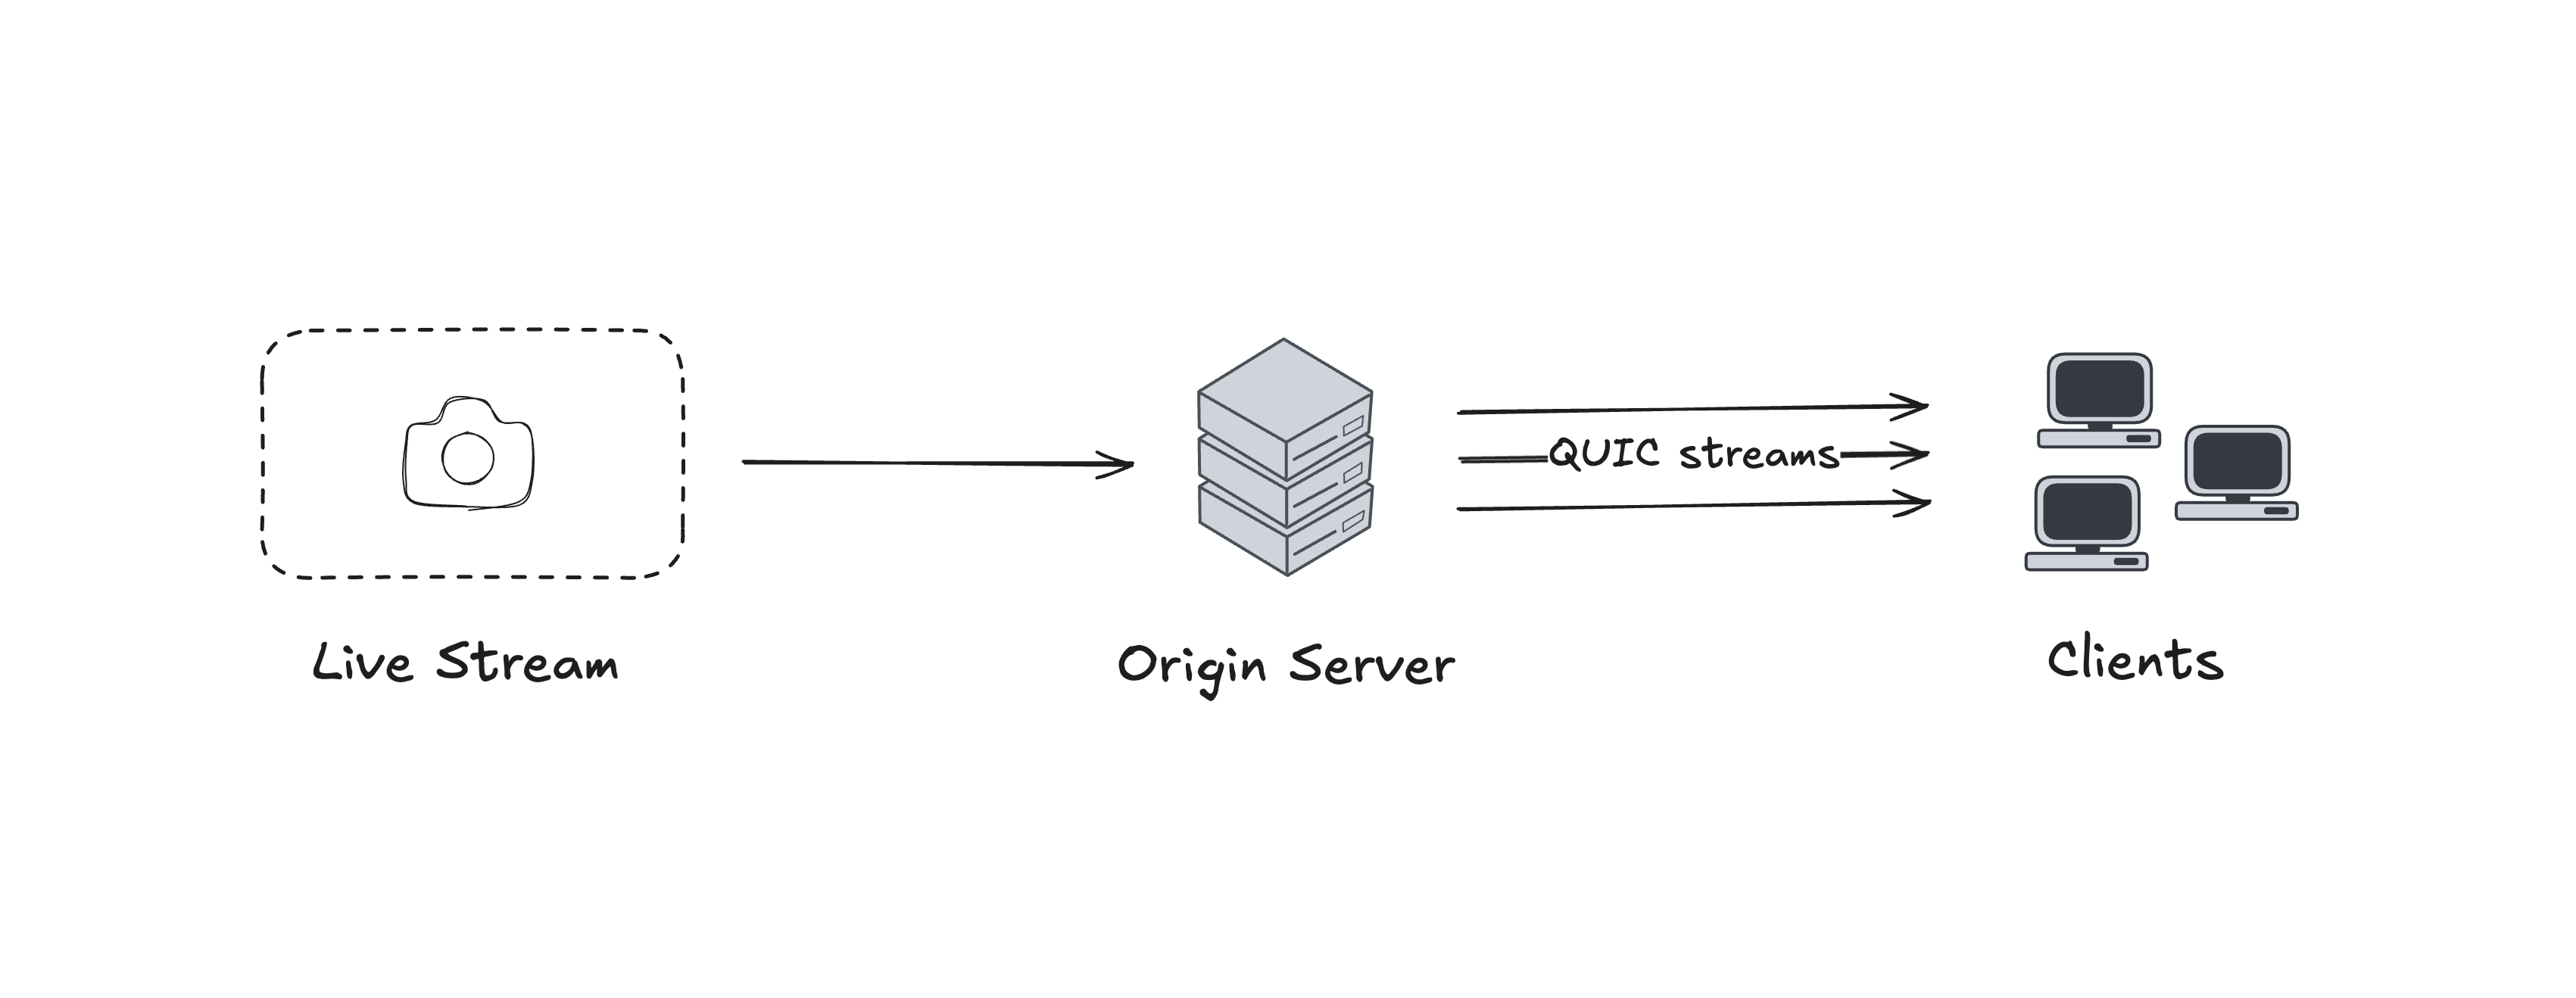
\includegraphics[width=\textwidth]{figures/architecture.png}
    \caption{Architecture of our prototype system}
    \label{fig:architecture}
\end{figure}

\section{Origin server}
The origin server serves a single broadcast. It uses two \ac{MoQ} tracks for this purpose: the \textit{init} track and the \textit{video} track. The init track is used to transmit the ftyp and moov boxes to clients, which contain the information that the client needs to parse the MP4 fragments and deocde the video frames. Similar to how clients in a \ac{HAS} system fetch the manifest file, clients subscribe to the init track on startup. The video track is used to serve the actual video content.

The origin server is implemented in Rust and uses moq-transport\footnote{\url{https://crates.io/crates/moq-transport}}, a Rust crate that implements the \ac{MOQT} protocol. The server ingests and broadcasts the stream as follows. First, the server creates a \lstinline{Track} for the init and video tracks. A \lstinline{Track} is an abstraction provided by moq-transport to fan-out MoQ objects to multiple subscriptions. Using the \lstinline{Track} API, an application writes objects to the track using a writer handle, and moq-transport notifies any readers reading the track using the reader handles. After creating the tracks, the server starts and executes two processes concurrently.

The server reads the video stream from standard input (stdin), parses the MP4 boxes and writes them to the respective \lstinline{Track}. First, the ftyp and moov boxes are ingested. The server writes a MoQ object containing both boxes to the init track. Following the ftyp and moov boxes, is a stream of moof and mdat boxes, with each pair corresponding to a MP4 fragment. The MP4 stream is fragmented at every frame with the ffmpeg option \lstinline{frag_every_frame}\footnote{\url{https://ffmpeg.org/ffmpeg-formats.html\#Options-6}}, so that each MP4 fragment contains a single video frame. If the frame contained in the MP4 fragment is a keyframe, the server creates a new MoQ group. Keyframes always introduce new MoQ groups so that clients can start subscriptions at the latest possible point in time, which is the start of the most recent group. For each fragment that is ingested, using a handle to the current group, the server writes an object to the video \lstinline{Track} with the fragment as the object's payload.

Simultaneously, the origin server listens to new subscription requests and serves existing subscriptions by broadcasting the local \lstinline{Track}. For each subscription request that the server receives, it creates an asynchronous, non-blocking \textit{task}, a form of a lightweight thread in Rust,  to serve the init or video track to the client. In this task, the server reads the MoQ objects from the local \lstinline{Track}, which are being written in the ingestion process, and transmits them to the client using the existing QUIC connection. To transmit the MoQ object, the server opens a new QUIC stream or uses an existing one, depending on the media to streams mapping configuration. Our baseline implementation transmits the frames reliably and in order, using a single QUIC stream, similar to a traditional live-streaming system that uses TCP. We explore other ways to map media to streams and prioritize these in chapters \autoref{chapter:deprioritizing_b_frames} and \autoref{chapter:skipping_old_media}.

% TODO: where should i put this?
% Our prototype uses draft version 3 of \ac{MOQT}, but the main points outlined in this section should be applicable to versions 4 and 5, the latest version at the time of writing.

\section{Live streaming client}\label{section:baseline_client}
% TODO: make sure to explain what the render pipeline is, and mention calculateTimeUntilFrame
We now turn our attention to the client.

Subscribing and playing a live stream works as follows. First, the client downloads the ftyp and moov boxes, by subscribing to the init track. These boxes contain metadata about the tracks in the MP4 stream % TODO: such as...
that the client will later need to parse the mp4 fragments and decode the video frames.

When the user clicks "play", the client subscribes to the video track. Since the player can't start playback in the middle of a GoP, the client can choose between two different locations for which the subscription should start. The client can either wait for the new GoP to be produced or subscribe to the latest GoP. Assuming a GoP to MoQ group mapping, like we do in our server, in MoQ draft 3 we can achieve the former by using the Subscribe location mode RelativeNext and value 0 and to achieve the latter, we use mode RelativePrevious and value 0. Waiting for the next GoP to start ensures the lowest possible latency, while starting playback at the latest GoP keeps startup delays low but it can lead to latencies up to the duration of GoPs. % TODO: this is not really true, because we can simply subscribe to the latest gop and flush all frames until the last frame or something like this
Whether to prioritize startup delay or latency is up to decide based on the use case.

As the client receives the MP4 fragments from the video track, it adds them to a pipeline that processes the raw fragments, extracting the video frames and eventually rendering them. The pipeline consists of three stages. 

First, the player extracts the frame payload and frame metadata such as the frame duration, decode timestamp and presentation timestamp from the mp4 fragment. 

Then we decode the encoded frame using the frame metadata with the VideoDecoder from the WebCodecs API. We configure the decoder using the ftyp and moov boxes, which we downloaded from the init track.  To configure the VideoDecoder, two options are worth mentioning. We enable \lstinline{optimizeForLatency} % TODO: What does optimizeForLatency actually do
and set \lstinline{hardwareAcceleration} to \lstinline{"prefer-software"}. Regarding the latter, with the default setting, the VideoDecoder was occasionally throwing errors with the message "Decoding error". With \lstinline{"prefer-software"} these errors did not occur, although we can't fully explain the reason behind it. % TODO: Elaborate. E.g. These errors could be caused by A deeper issue with our implementation could We are not sure if this is an issue with our implementation or an issue with the WebCodecs API.

Finally, we render the decoded frame, by drawing it to a canvas element. Rendering frames as they are received results in jerky playback, and consequently poor \ac{QoE}. To provide smooother playback, we use a jitter buffer and time the rendering of frames, rather than rendering the frames immediately after decoding them. After a frame is received and decoded, it is added to the jitter buffer. Once the buffer size reaches the target size, the player start consuming frames from the buffer. While the buffer has frames, the player continually retrieves the frame with the lowest timestamp from the buffer, and waits for the correct time to render it. If the buffer runs out of frames, the player starts the process of filling the buffer again.

% TODO: explain the algorithm. Explain that resumedPlayingAt is set to undefined when the player first starts, or rebuffers, and that it's set when the first frame is rendered after a pause, or rebuffer event
Algorithm \ref{alg:time_until_frame} shows how the player calculates the time until a frame is to be rendered. The time the player should wait depends on the current media time, which is the elapsed time since playback started in the current session. If the stream can be played without interruptions, the time until a frame is to be rendered is the difference between the frame timestamp and the media time. However, if the player rebuffers, using the absolute media time would cause all frames that are lagging behind to be rendered immediately after the player resumes playback at the same. If the network conditions that led to the rebuffering event are not short-lived, then the player would continuously flush all frames, emptying the buffer, and start buffering again. We handle this issue, by timing the rendering of frames relative to the point in time, at which playback resumed after a rebuffering event, rather than the absolute playback start.  % TODO: However if we do this, it increases latency. Further work needs to be done on this. Find a hybrid strategy

% TODO: Explain that latency keeps increasing if we do this. 
% TODO: Explain that when network recovers and we get a bunch of media we can skip old media by checking if the buffer did grow past a threshold

\begin{algorithm}
\caption{Calculate time to render frame}\label{alg:time_until_frame}
\begin{algorithmic}
\Function{calculateTimeUntilFrame}{$frameTimestamp$}
    \State $now \gets \Call{now}{\null}$
    \item[]
    \If{$resumedPlayingAt = undefined$}
        \State $resumedPlayingAt \gets \textnormal{\{\}}$
        \State $resumedPlayingAt.localTime \gets now$
        \State $resumedPlayingAt.mediaTime \gets frameTimestamp$
    \EndIf
    \item[]
    \State $relativeMediaTime \gets now - resumedPlayingAt.localTime$
    \State $relativeFrameTimestamp \gets \newline
        \hspace*{3em}(frameTimestamp - resumedPlayingAt.mediaTime) / 1000$
    \State \Return $\max(0, relativeFrameTimestamp - relativeMediaTime)$
\EndFunction
\end{algorithmic}
\end{algorithm}


\section{Deprioritizing B-frames}\label{chapter:deprioritizing_b_frames}
In order to prevent the latency from increasing during network congestion, the server needs to send less data to the client. One way to reduce the stream's bitrate is by dropping B-frames. The reason this works is twofold. 

First, B-frames are not usually depended by other frames, and therefore they can be dropped without affecting the decodability of other frames. We will assume for the remainder of this section that B-frames are not used as references. We note however that state of the art encoders allow the use of B-frames as references through B-pyramid schemes. We will discuss the use of reference B-frames, including ways to adapt our implementation to support them, towards the end of the section. % TODO: Can B-frames be used in low-latency livestreaming

Second, the P-, and I-frames alone form themselves a stream that is playable, albeit with video artifacts, such that we can drop all B-frames if necessary. This is only true, if the number of consecutive B-frames is limited, which is the case in low-latency live streaming. % TODO: explain why: since dropping too many frames in a row would result in an incoherent video. If this were not the case, then it would like we were skipping media. This is a viable strategy, but it's one that requires different ways to render the frames at the client. We will talk about this in the next section.

% TODO: cite https://www.ietf.org/id/draft-lcurley-moq-transfork-00.html#name-layers?
We effectively divide the stream into two layers: a base layer, consisting of the I-, and P-frames, and an enhancement layer containing all B-frames. During congestion, the server drops the enhancement layer, degrading the stream quality to reduce the stream's bitrate.


% TODO: find a better name for this section
\subsection{Implementation}
Our goal is to deprioritize the B-frames, such that they are sent on a best-effort basis. To accomplish this, we prioritize the layers as follows. The base layer is assigned the highest priority so that the server always transmits I-frames and P-frames first, if any are available. On the other hand, B-frames get a lower priority, such that they are transmitted only if there is enough network bandwidth.

We divide the stream into two MoQ tracks, one for each layer. In both tracks each GoP forms a group. The group boundaries must be aligned in this way to provide a join point for new subscriptions that is synchronized across both tracks. The server implements this by incrementing the groupId for each keyframe. At startup, the client subscribes concurrently to both tracks referencing the same MoQ group.

The track that serves the base layer uses a single QUIC stream to deliver the I- and P-frames in order. 
% TODO: mention that we are using quinn-rs and how it implements priorities
We assign the second highest priority to this stream. (The highest priority value is assigned to the
init track).

% TODO: Maybe use an excalidraw sketch to make the explanation more clear
To stream the enhancement layer, one could think of using a single stream with a lower priority. However, this simple prioritization strategy wouldn't have the desired effect. We demonstrate the issue with an example. Suppose that the network was congested and we didn't transmit any B-frames because there wasn't enough bandwidth. When the network recovers, we want to transmit the new B-frames. However the old B-frames are transmitted because they were queued first. If the network has just enough bandwidth to send the B-frames of one GoP, we would never get a chance to render the B-frames. They would always be late. The same reasoning applies to a stream per GoP for the B-frames. If the server gets enough bandwidth to transmit some B-frames towards the end of a GoP, we don't want to send the first frames of the GoP since they are useless. 

Each B-frame should have a higher priority than the previous B-frame that was produced. In general, frames in enhancement layers should be prioritized according to the new over old policy, since they are always transmitted on a best-effort basis. 

Since, in QUIC, the unit of prioritization is the stream, each B-frame needs to be sent in a separate stream. The decode timestamps of B-frames can be used as the priority for each stream, or if one wants to make optimal use of the number of bits, the current count of B-frames.

% TODO: fix this. a single frame can contains slices of all types
To prioritize I-, and P-frames over B-frames, the server must be able to distinguish frames of different types in the first place. Identifying the type of a frame is not as trivial as one might think. Parsing the mp4 fragments is not enough, because there doesn't exist any boxes in the mp4 container that contain this information. One needs to parse the encoded sample. For AVC encoded frames, for example, we first parse the \ac{NAL} units with the type 0, Coded slice of a non-IDR picture, and type 5, Coded slice of an IDR picture, from the mp4 sample. We then parse the slice types from the slice header of these NAL units.

Additionally, the server includes the frame type in the header of the payload of the MoQ object, such that clients, and potentially relays as well, can easily extract the type of a frame from the MoQ object without having to parse the encoded samples.

\subsection{Handling out-of-order frames}\label{section:out_of_order_frames}
% TODO (maybe): instead of explaining why they can arrive out-of-order, simply say that is best to assume they will arrive out-of-order because nothing guarantees that they will arrive in order when we use multiple streams
Because we are using multiple QUIC streams, which are independent and don't provide any ordering guarantees, frames will arrive out-of-order. Within the base layer, I- and P-frames will arrive in decode order, however B-frames can arrive out-of-order relative to the frames in the base layer. Furthermore, B-frames can arrive out-of-order relative to each other. First, if the network becomes temporarily congested such that some B-frames are not transmitted, then old B-frames will be sent to the client when the network recovers. Second, a B-frame can arrive ahead of another B-frame that was sent first, because the underlying packets take different network paths or due to packet loss. % TODO: cite source
In this subsection, we propose a solution to this issue. First, we explain the intuition behind our approach, and then we describe it more precisely, by explaining relevant implementation details.

% TODO: explain what the render pipeline is (in the baseline version section)
We add frames from the base layer, which arrive in order relative to each other, directly to the render pipeline. Although there might be discontinuities between these frames, we don't wait for the missing B-frames, because they might never arrive.

B-frames can be late or early. We define a B-frame to be late, if at the time of its arrival a frame with a higher timestamp has already arrived. Similarly we say a B-frame is early, if it arrived ahead of frames with a lower timestamp. If a B-frame is late, we drop it, because we don't want to decode and render frames out-of-order. If a B-frame is early and no later I-, or P-frames have arrived, we wait for the earlier frames to arrive. This is because the B-frame might have arrived ahead of a frame from the base layer, which we can't drop. Note that the B-frame might simply be ahead of other B-frames, but we have no way of telling, so we need to assume the worst case. If a B-frame is neither late nor early by our definitions, we add it directly to the render pipeline. 

In practice, frames that are in order are not added directly to the render pipeline. Instead frames are first added to a jitter buffer to handle small variations in the arrival of frames. Otherwise, if we add frames directly to the render pipeline, a frame that is late by only a few milliseconds will be dropped. From our experiments, we found a 100 to 200 milliseconds jitter buffer to be optimal. % optimal in what sense? explain

% TODO: double check correctness of the algorithm and reasoning
% TODO: explain that buffer works like a priority queue, and buffer[0] is the frame with the lowest decode timestamp and buffer[buffer.length - 1] is the frame with the highest timestamp
% Explain the bufferSize function?
% explain why you use a while loop instead of an if statement
Algorithm \ref{alg:reorder} shows pseudocode for the process of handling an incoming frame and retrieving the next frame to be enqueued to the render pipeline. In summary: first, we check if the frame is a B-frame and if the frame is late, by checking if it has a lower decode timestamp than the decode timestamp of the last enqueued frame. If the B-frame is late, we drop it. Otherwise, we add the frame to the jitter buffer. This buffer works like a min-heap with the decode timestamps serving as the key. Then, if the buffer size is greater than the target size, we \textit{try} to retrieve the next frames from the buffer and enqueue them to the render pipeline. To do this, we check the frame with the lowest timestamp in the buffer. If the frame is an I-, or P-frame or if there is no discontinuities between the frame's dts and the last enqueued frames dts, we enqueue the frame to the buffer and try to enqueue the next frame. If the frame is a B-frame and it is early, then we scan the buffer for an I-, or P-frame. If we find an I-, or P-frame, then it must be the case that the frame has a higher timestamp, and we enqueue the frame. Note that the B-frame cannot be ahead of any I-, or P-frames since frames from the base layer are transmitted in order. If, on the other hand, the buffer only has B-frames, then we wait for the missing frames to arrive by returning, since it might be ahead of I-, or P-frames.

\begin{algorithm}
\caption{Reorder Algorithm}\label{alg:reorder}
\begin{algorithmic}
\Function{reorder}{$frame$}
    \If{$frame.type = B \land lastEnqueued \neq null \land frame.dts < lastEnqueued.dts$}
        \State \Return \Comment{Drop late B-frames}
    \EndIf
    \item[]
    \State add $frame$ to $buffer$
    \item[]
    \While{$\Call{bufferSize}{\null} > targetSize$}
        \State $next \gets buffer[0]$
        \If{\newline
            \hspace*{4.5em}$next.type \neq B \lor \newline
            \hspace*{4.5em}lastEnqueued = null \lor \newline
            \hspace*{4.5em}next.dts = lastEnqueued.dts + lastEnqueued.duration$\newline\hspace*{2.7em}}
            \State enqueue $next$
            \State pop $buffer$
            \State $lastEnqueued \gets next$
            \State \textbf{continue}
        \EndIf
        \item[]
        \State $i \gets 1$ \Comment{B-frame is early}
        \While{$i < buffer.length \land buffer[i].frameType = B$}
            \State $i \gets i + 1$
        \EndWhile
        \If{$i < buffer.length$} \Comment{B-frame is not ahead of any I-, or P-frames}
            \State enqueue $next$
            \State pop $buffer$
            \State $lastEnqueued \gets next$
        \Else \Comment{Wait, because B-frame might be ahead of I-, or P-frames}
            \State \textbf{break} 
        \EndIf
    \EndWhile
\EndFunction
% \item[]
% \Function{bufferSize}{\null}
%     \If{$buffer.length = 0$}
%         \State \Return 0
%     \EndIf
%     \item[]
%     \State $oldest \gets buffer[0]$
%     \State $newest \gets buffer[buffer.length - 1]$
%     \State \Return $newest.dts - oldest.dts$
% \EndFunction
\end{algorithmic}
\end{algorithm}

\subsection{Reference B-frames}\label{section:reference_b_frames}
We assumed until now that B-frames are not depended on by other frames. However, H.264 and newer video codings allow B-frames to be used as references for the encoding of other frames. Dropping a B-frame that is used as a reference, while trying to decode the dependent frames, will cause video distortions. A decoder can't decode a frame without its dependencies without errors. The approach we described so far doesn't distinguish between reference and non-reference B-frames and therefore video distortions will occur when the network is congested.

The simplest solution is to disable the use of B-frames as references, at the cost of a slighly lower coding efficiency. For AVC/H.264, one can control this with the b-pyramid setting\footnote{\url{https://en.wikibooks.org/wiki/MeGUI/x264\_Settings\#b-pyramid}}. In live streaming, the decrease in coding efficiency resulting from disabling this option is limited, since we use a relatively low number of B-frames.

However one might not be able to configure the encoder settings. A production live streaming platform for example might ingest streams from a variety of sources, of which the user is in control of the encoding configuration. In these cases, one must design a streaming protocol that handles reference B-frames properly.

One approach consists in distinguishing reference from non-reference B-frames and transmit reference B-frames together with the I-, and P-frames. In the client we wait for any reference B-frames, if a non-reference B-frame arrives early just like we do for I-, and P-frames. This ensures that reference B-frames are not dropped and therefore we don't cause video distortions. To identify the reference B-frames, one can try using the mp4 sample flags \lstinline{sample_depends_on} and \lstinline{sample_is_depended_on}. % TODO: cite mp4 spec
We note, however, that in our experiments, both flags were set to the value $0$, indicating that the dependencies were unknown, for the majority of frames. We weren't able to find an explanation for this. One can also try identifying reference B-frames by parsing the \ac{NAL} units of the AVC encoded stream. 

We propose a different approach that doesn't require knowing precisely which B-frames are used as references. This approach is based on the observation that B-frames with a lower decode order are more likely to be referenced by other B-frames. Recall that, whenever a frame depends on a future frame, which is the case with B-frames or bi-directional predicted frames, the future frame is encoded first, and therefore has a lower decode timestamp. Frames only depend on frames with a lower decode order. 

\begin{figure}
    \centering
    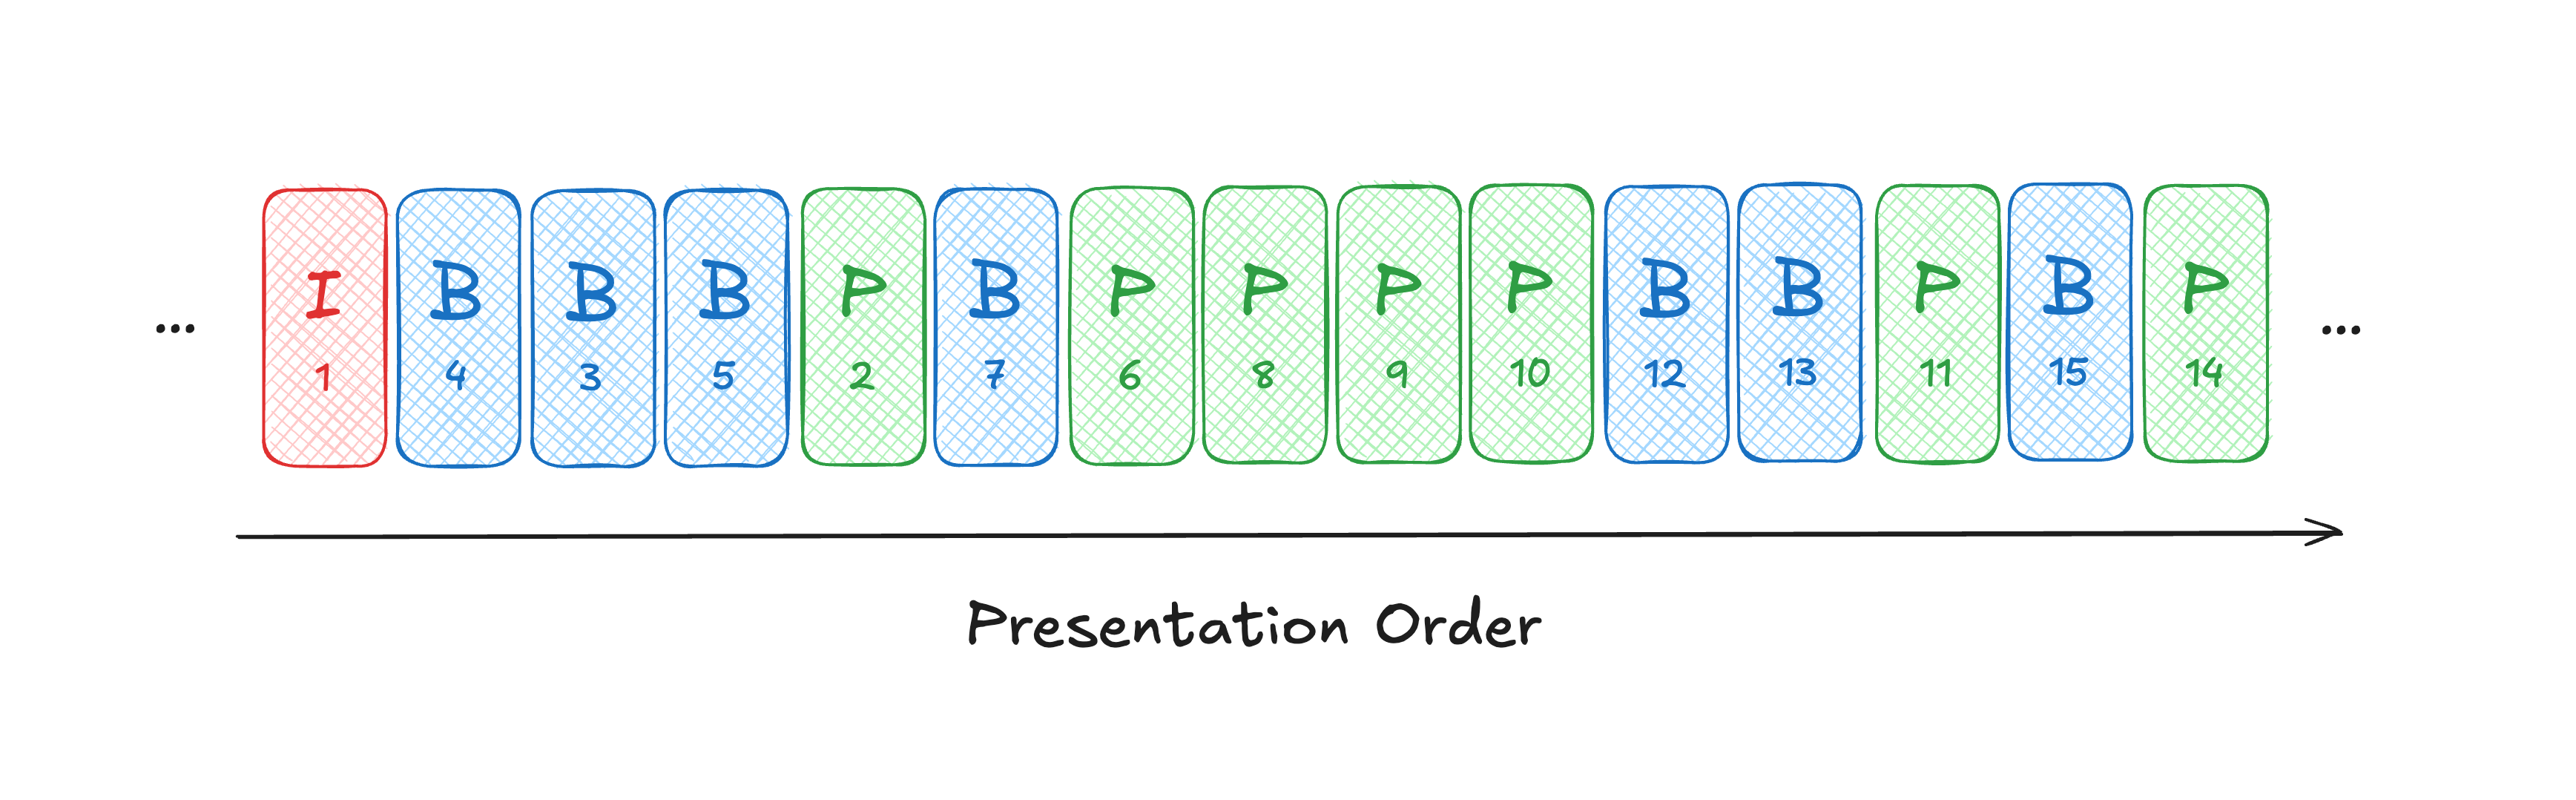
\includegraphics[width=\textwidth]{figures/gop_structure.png}
    \caption{Example \ac{GoP} with frames and their decode order}
    \label{fig:gop_structure}
\end{figure}

We found this heuristic to work well for \ac{GoP} structures with a maximum of three B-frames between between each I-, or P-frame. We haven't tested \ac{GoP} structures which use more than three B-frames, since using more than three B-frames is not common in low-latency live streaming. From our experiments, we observed that when there were consecutive B-frames, the first two frames were always out of order, as we can see in the first group of B-frames in \autoref{fig:gop_structure}. This indicates that the second B-frame is being used as a reference by the first B-frame, otherwise the two frames wouldn't be out of order. Furthermore, dropping only the second B-frame caused very noticable video distortions, both for the first and third frames in the group, as shown in \autoref{fig:video_artifacts}. We conclude that in addition to the first B-frame, the third B-frame also depends on the second B-frame. On the other hand, dropping the second and third B-frames didn't cause any video distortions, and therefore we assume that these frames are not used as references. With less than three consecutive B-frames, none was used as a reference in our experiments.

% Recall that B-frames, bi-directional predicted frames, reference both a preceding frame and a future frame. For this reason, future frames that are depended by B-frames come before than the B-frames that reference it. 

\begin{figure}
    \centering
    \begin{subfigure}{\textwidth}
        \centering
        
\includegraphics[width=0.3\textwidth]{figures/video_artifacts/all_frames/frame_00167.png}
        
\includegraphics[width=0.3\textwidth]{figures/video_artifacts/all_frames/frame_00168.png}
        
\includegraphics[width=0.3\textwidth]{figures/video_artifacts/all_frames/frame_00169.png}
        \caption{Original frames}
    \end{subfigure}

    \vspace{1em}

    \begin{subfigure}{\textwidth}
        \centering
        
\includegraphics[width=0.3\textwidth]{figures/video_artifacts/drop_first_b_frame/frame_00149.png}
        
\includegraphics[width=0.3\textwidth]{figures/video_artifacts/drop_first_b_frame/dropped.png}
        
\includegraphics[width=0.3\textwidth]{figures/video_artifacts/drop_first_b_frame/frame_00150.png}
        \caption{Frames decoded without the second B-frame}
    \end{subfigure}
    \caption{Video artifacts caused by dropping the second B-frame of a group of three consecutive B-frames}
    \label{fig:video_artifacts}
\end{figure}

Since B-frames with a lower decode order are more likely to be used as references, we prioritize older B-frames over newer ones within a group of consecutive B-frames, so that frames which are depended on are more likely to be delivered first. We will use the term B-frame group to denote a group of consecutive B-frames. Across B-frame groups, we use the same new over old policy, by assigning a higher priority to newer groups. Note, however, that AVC/H.264 allows P-frames to reference B-frames. As a result, video distortions will still occur, whenever a B-frame that is referenced by a P-frame is dropped.

% An alternative is to transmit reference B-frames with a lower priority than I-, and P-frames, but with a higher priority than non-reference B-frames. This is a sensible approach, particularly when the encoder uses a \ac{GoP} structure, in which reference B-frames are only refenced by other B-frames. To minimize video distortions, we still drop non-reference B-frames if the   Furthermore, we drop non-reference B-frames if the respective reference B-frame hasn't arrived. This is based on the observation that skipping the rendering of the other B-frames has a much less noticeable impact on video quality than rendering the two B-frames with video distortions.


% The  The drawback is that we can't fully eradicate video distortions, since P-frames can also reference B-frames. However, only a few P-frames reference B-frames and the impact of dropping the reference B-frame is much smaller, because they reference much less macroblocks of the B-frame, and therefore the impact on the frame is much lower, as shown in the P-frame in \autoref{fig:video_artifacts}. 

% We implement this priority scheme as follows. Let $P_k \in [0, P_{max}]$ be the priority of frame $k$. $P_k$ can be formulated as:

% \begin{align*}
%     P_k &= P_{max}, & \text{if } k \text{ is an I-, or P-frame} \\
%     P_k &= (G_k \ll b) + 2^b - I_k, & \text{if } k \text{ is a B-frame}\\
% \end{align*}

\section{Skipping old media}\label{chapter:skipping_old_media}
Adapting a live stream's quality is an effective technique for prioritizing latency, but it can't handle large changes in the network bandwidth effectively alone. Consider the case where a viewer is watching a live stream on their phone and the available network bandwidth drops drastically and then recovers. This can happen because the viewer is watching the live stream on his phone on the go and temporarily goes past an area of bad coverage for example. While the network connectivity is poor, streaming a lower quality stream surely helps. However video will still lag behind and latency will increase, due to the low network throughput. Video will queue up at the server. When the network recovers, rather than playing all the video that queue up, we want to resume playback at the live edge. We want to skip large portions of media if we don't get a chance to transmit it due to network conditions.

% TODO: mention Warp
To achieve this, we prioritize new over old media. 

Specifically, we map and prioritize the video track as follows. We map each GoP of the video stream to a MoQ group, and send each group in its own QUIC stream. We prioritize new GoPs over old ones, by using the timestamp of the first frame in the group as the priority of the QUIC stream.

In the client, we drop any frames belonging to old GoPs. Handling late GoPs is similar to how we handled out-of-order frames in \autoref{section:out_of_order_frames}. One can keep track of the last frame that we enqueued to the processing pipeline and compare the timestamps of new frames with the timestamp of this frame, dropping the new frames if they have a lower timestamp. % TODO: Note that as opposed to subsection 2.2.2, we don't use a jitter buffer, because it doesn't make sense % TODO: Explain why

% TODO: find a better name
\subsection{Snapping video forward}\label{section:snapping_video_forward}
Our goal is to render new media immediately, such that plackback jumps from the old media forward to the new media. Recall, however, that the player, as we first described in \autoref{section:baseline_client}, times the rendering of frames using the relative frame timestamp. Using Algorithm \ref{alg:time_until_frame} to time the rendering of new media, would lead to the player waiting for the frame's timestamp before rendering the new GoPs, and thereby not decreasing the latency. On the one hand, we want to render new media immediately. On the other hand, we want to buffer and time consecutive frames according to their presentation time for smoother playback. To achieve this, we compare the presentation timestamp of the previously rendered frame and the frame that we are about to render. If there is a discontinuity between the presentation timestamps, we render the frame immediately, otherwise we time the rendering of the frame.

To implement this, the client keeps track of the timestamp of the last frame that was rendered and we adapt Algorithm \ref{alg:time_until_frame}, so that it first checks if there is a discontinuity between $frameTimestamp$ and the timestamp of the last rendered frame. If there is a discontinuity, $calculateTimeUntilFrame$ returns 0, so that the frame is rendered immediately. Note that if there is a discontinuity, we also need to update $resumedPlayingAt$ so that we use the correct media time as the reference when timing the next frames.

% TODO: Implement it, and measure it properly. Expand on this idea. If i do end up doing this, turn this into its own chapter.
\section{Combining both strategies}
Ideally, we want the live streaming system to handle both small drops in the network bandwidth and short spikes effectively. Although, we haven't had the time to test our hypothesis, we believe that combining both approaches lead to the most optimal performance. In this section, we describe how we would combine deprioritize B-frames and skip old GoPs. We begin by presenting a new priority scheme that integrates the new over old policy with the priority scheme of deprioritize B-frames. We then propose a way to time frames in the client.

Just like in \autoref{section:deprioritizing_b_frames} we create a track for the I-, and P-frames and a track for the B-frames. Now instead of using a stream per track for the base layer, we use a stream per GoP, and prioritize new GoPs over old GoPs. Again, we must assign the highest priorities to the streams in the base layer. For this purpose, we divide the value range of the priority values into two ranges. The values in the highest range are for the streams in the base layer, while the lowest range is for the B-frames. To make optimal use of the available bits, one can allocate more bits for the latter, since the number of B-frames is in general higher than the number of GoPs.

We would like to note that we are aware that this approach might not be viable with certain QUIC implementations, because the prioritization implementation does not use enough bits. quinn-rs for example uses 32 bits for the priority value. These are not enough bits for long duration streams. % TODO: Give a back-of-the-envelope calculation type of example

Regarding the client, we use the approach described in \ref{section:snapping_video_forward} with a small modification. Rather than rendering frames instantly if there is any discontinuity, we time frames if the discontinuity is bigger than a predefined threshold. This is because frames from the base layer might have discontinuities, if we drop B-frames, and we don't want to render them immediately. % TODO: Expand on this. The question is what's the threshold? When are two frames too far apart, such that we should render the later frame instantly. % TODO: Finish this part

% !TeX root = ../main.tex
% Add the above to each chapter to make compiling the PDF easier in some editors.

\chapter{Evaluation}\label{chapter:evaluation}
We now turn to the evaluation of the streaming protocols we presented, referred to in this chapter as deprioritize B-frames and skip old \acp{GoP}. We begin by describing the testbed and metrics used to measure the performance of our streaming protocols. Then, we present the results collected from multiple test runs of our approaches across different network profiles. We conclude with a qualitative evaluation, in which we discuss additional factors that should be accounted for when considering either approach.

\section{Testbed}
Our testbed emulates network bandwidth limits during a live streaming session between the client and the origin server. We perform multiple test runs for each streaming protocol, in which we first launch the client, establish a connection to the server, and subscribe to the video stream. Once playback starts, we simulate various types of network patterns that are representative of real-world network conditions and collect relevant metrics. The network profiles used, which are taken from Twitch's 2020 Grand Challenge on low-latency live streaming \parencite{twitchGrandChallengeAdaptation}, are shown in \autoref{fig:bandwidth_profiles}.

\begin{figure}
    \centering
    
    % First row - Cascade profiles
    \begin{subfigure}[b]{0.3\textwidth}
        \centering
        \begin{tikzpicture}
            \begin{axis}[
                width=\textwidth,
                % xlabel={Time (s)},
                % ylabel={Bandwidth (Kbit/s)},
                ymin=0, ymax=1300, ytick distance=200,
                ymajorgrids=true,
                grid style=dashed,
                tick label style={font=\footnotesize},
                label style={font=\footnotesize},
            ]
            \addplot[red, const plot, thick, solid, mark=*] coordinates {
                (0,1200) (30,1200) (30,800) (60,800) (60,400) (90,400)
                (90,800) (120,800) (120,1200) (150,1200)
            };
            \end{axis}
        \end{tikzpicture}
        \caption{\footnotesize CASCADE}
    \end{subfigure}
    \begin{subfigure}[b]{0.3\textwidth}
        \centering
        \begin{tikzpicture}
            \begin{axis}[
                width=\textwidth,
                % xlabel={Time (s)},
                % ylabel={Bandwidth (Kbit/s)},
                ymin=0, ymax=1300, ytick distance=200,
                ymajorgrids=true,
                grid style=dashed,
                tick label style={font=\footnotesize},
                label style={font=\footnotesize},
            ]
            \addplot[red, const plot, thick, solid, mark=*] coordinates {
                (0,1000) (15,1000) (15,800) (30,800) (30,600) (45,600) (45,400) (60,400)
                (60,200) (75,200) (75,400) (90,400) (90,600) (105,600) (105,800) (120,800)
                (120,1000) (135,1000)
            };
            \end{axis}
        \end{tikzpicture}
        \caption{\footnotesize INTRA\_CASCADE}
    \end{subfigure} 

    \vspace{1em}
    
    % Second row - Other profiles
    \begin{subfigure}[b]{0.3\textwidth}
        \centering
        \begin{tikzpicture}
            \begin{axis}[
                width=\textwidth,
                % xlabel={Time (s)},
                % ylabel={Bandwidth (Kbit/s)},
                ymin=0, ymax=1300, ytick distance=200,
                ymajorgrids=true,
                grid style=dashed,
                tick label style={font=\footnotesize},
                label style={font=\footnotesize},
            ]
            \addplot[red, const plot, thick, solid, mark=*] coordinates {
                (0,500) (0.25,500) (0.25,1200) (5.25,1200) (5.25,500) (5.35,500)
                (5.35,1200) (6.35,1200) (6.35,500) (6.6,500) (6.6,1200) (11.6,1200)
            };
            \end{axis}
        \end{tikzpicture}
        \caption{\footnotesize FAST\_JITTERS}
    \end{subfigure}
    \begin{subfigure}[b]{0.3\textwidth}
        \centering
        \begin{tikzpicture}
            \begin{axis}[
                width=\textwidth,
                % xlabel={Time (s)},
                % ylabel={Bandwidth (Kbit/s)},
                ymin=0, ymax=1300, ytick distance=200,
                ymajorgrids=true,
                grid style=dashed,
                tick label style={font=\footnotesize},
                label style={font=\footnotesize},
            ]
            \addplot[red, const plot, thick, solid, mark=*] coordinates {
                (0,500) (5,500) (5,1200) (10,1200) (10,500) (15,500) (15,1200) (20,1200)
                (20,500) (25,500) (25,1200) (30,1200)
            };
            \end{axis}
        \end{tikzpicture}
        \caption{\footnotesize SLOW\_JITTERS}
    \end{subfigure}
    \begin{subfigure}[b]{0.3\textwidth}
        \centering
        \begin{tikzpicture}
            \begin{axis}[
                width=\textwidth,
                % xlabel={Time (s)},
                % ylabel={Bandwidth (Kbit/s)},
                ymin=0, ymax=1300, ytick distance=200,
                ymajorgrids=true,
                grid style=dashed,
                tick label style={font=\footnotesize},
                label style={font=\footnotesize},
            ]
            \addplot[red, const plot, thick, solid, mark=*] coordinates {
                (0,1200) (10,1200) (10,300) (20,300) (20,800) (30,800)
            };
            \end{axis}
        \end{tikzpicture}
        \caption{\footnotesize SPIKE}
    \end{subfigure}

    \vspace{1em}

    \caption{Bandwidth profiles - Bandwidth (Kbit/s) vs. time (s)}
    \label{fig:bandwidth_profiles}
\end{figure}

We use dummynet\footnote{\url{https://man.freebsd.org/cgi/man.cgi?dummynet}} to emulate a link with limited bandwidth between the origin server and the client. Dummynet is a traffic shaping tool that simulates queue size and bandwidth limitations, delays, and packet loss by intercepting traffic between the transport protocol layers \parencite{rizzoDummynetSimpleApproach1997}. % TODO: I can expand on how it works if i want
In order to simulate the bandwidth limits, we use a dummynet \textit{pipe} and feed traffic from the client to the server and vice versa into the pipe using PF\footnote{\url{https://www.openbsd.org/faq/pf/}} (Packet Filter).

The client and origin server run on the same machine and communicate through the loopback interface. The origin server listens for incoming QUIC connections on port 443. We use PF rules that filter traffic on the localhost address from port 443 to any port, which corresponds to traffic between the server and the client, and forward it to the dummynet pipe. The dummynet pipe is configured with a bandwidth limit that varies according to the network profile throughout the test run. We don't configure any other options of the dummynet pipe explicitly so that their default values are used. Some options worth mentioning include the queue size, which is set to 50 slots or packets by default, and the delay, which is zero if not configured explicitly.

For the source video stream, we use the Big Buck Bunny\footnote{\url{https://peach.blender.org/}} video and read the input file at the native frame rate using the FFmpeg option \lstinline{-re} to simulate live streaming. The video frame rate is 24 frames per second. We also reencode the video stream with H.264/AVC using a custom bitrate and GoP structure and repackage it in MP4 fragments. We use the following FFmpeg options to achieve this:
\begin{itemize}
    \item \lstinline{-an}: discard the audio track.
    \item \lstinline{-c:v libx264 -b:v 600k -bufsize 200K}: reencode the video using a target bitrate of 600 Kbit/s and a buffer size of 200 Kbit/s. The libx264 encoder is used.
    \item \lstinline{-g:v 15 -keyint_min:v 15 -sc_threshold:v 0}: set the minimum and maximum GoP size to 15 frames and disables scene change detection so that each GoP has exactly the same size. 
    \item \lstinline{-bf 3}: set the maximum number of consecutive B-frames to 3. Note that the encoder can use a lower number of B-frames between two reference frames.
    % \item \lstinline{-x264-params b-pyramid=none}: disable the use of B-frame as references for other frames to prevent video artifacts. The decoder produces video artifacts when it doesn't have a frame's dependencies as we described in \autoref{section:reference_b_frames}.
    \item \lstinline{-f mp4 -movflags cmaf+frag_every_frame}: use \ac{CMAF} compatible fragmented MP4 as the output format and package each frame in a separate fragment.
\end{itemize}

In both the deprioritize B-frames, and skip old \acp{GoP} approaches, we use a buffer size of 100 ms for the jitter buffer. Furthermore, in the deprioritize B-frames approach, the reorder buffer has a size of 100 ms, leading to a total buffer size of 200 ms. It is also worth mentioning that the server uses the BBR congestion control algorithm.

\section{Metrics}
We measure the latency of the live stream to evaluate the performance of our streaming protocols in poor network conditions. In a real-world live streaming system, many components in the media streaming pipeline contribute to the end-to-end latency \parencite{bentalebOneSecondLatencyEvolution2023}. In our measurements, we only take into account the latency added by the delivery and consumption phases since our work focuses on the media distribution phase of the pipeline. We measure latency as the delay between the frame reaching the server and being rendered in the client.  

% TODO: maybe cite where you got this idea from (dash player or twitch challenge testbed)
We measure the latency for each frame as follows. The server includes the availability time, the time at which the frame became available in the server, in the header of the MoQ object's payload. In the client, we calculate the latency for a given frame when the frame is rendered as the difference between the availability time and the time at which the frame was rendered. Note that both the server and client use the same clock, since they run on the same machine, and therefore clock drift is not an issue.

We would like to note however, that latency is not a complete metric by itself. Other factors, such as rebuffering events and stream quality, are also important in determining the viewer's \ac{QoE}. An interesting area for future work is to use a weighted combination of these factors, such as the \ac{QoE} model proposed by \citeauthor{yinControlTheoreticApproachDynamic2015} in \parencite{yinControlTheoreticApproachDynamic2015} to evaluate our approaches.

\section{Measurements}
We now present our results. First, we analyze the deprioritize B-frames approach, using measurements from two sample runs for the profiles 500 Kbit/s and INTRA-CASCADE. Next, we examine the skip old GoPs approach, reviewing measurements from a sample run. Finally, we show the average latency of each approach across multiple test runs for all profiles.

Deprioritizing B-frames results in lower latencies when the network bandwidth is slightly below the bitrate of the video stream. \autoref{fig:deprioritizing_b_frames_500Kbit:latency} shows the latency of each frame over time for sample runs of baseline and deprioritize B-frames. The bandwidth is limited to 500 Kbit/s, which is 100 Kbit/s below the average bitrate of the encoded video stream. At the start of the test run, the latency for both versions is similar. However, around 0:40, they begin to diverge, with deprioritize B-frames showing a slower rise in latency compared to baseline. The gap between the two versions increases steadily, reaching around 5 seconds at the 1:30 mark.

\begin{figure}
    \centering
    \begin{subfigure}{\textwidth}
        \centering
        \begin{tikzpicture}
    \begin{axis}[
    axis lines=left,
    ylabel=Latency (ms),
    legend style={at={(0.98,0.02)}, anchor=south east, draw=none},
    legend cell align=left,
    scaled ticks=false,
    ymin=0, ymax=25000,
    xtick distance=0.5, minor x tick num=1,
    x filter/.code={\pgfmathparse{#1/60}}, % Convert seconds to minutes
    xticklabel={ % Split into hours and minutes
        \pgfmathsetmacro\hours{floor(\tick)}%
        \pgfmathsetmacro\minutes{(\tick-\hours)*0.6}%
        % Use some trickery to get leading zeros
        \pgfmathprintnumber{\hours}:\pgfmathprintnumber[fixed, fixed zerofill, skip 0.=true, dec sep={}]{\minutes}%
    },
    ]
    
    \addplot+[only marks] table[meta=latencyMs] {data/sample_runs_gop15/500Kbit/baseline/latency_per_sec.dat};
    \addplot+[only marks] table[meta=latencyMs] {data/sample_runs_gop15/500Kbit/b_frames/latency_per_sec.dat};
    
    \legend{Baseline, Deprioritizing B-frames}
    
    \end{axis}
\end{tikzpicture}
        \caption{Latency}
        \label{fig:deprioritizing_b_frames_500Kbit:latency}
    \end{subfigure}

    \vspace{1.5em}

    \begin{subfigure}{\textwidth}
        \centering
        \centering
\begin{tikzpicture}
    \begin{axis}[
    width=0.48\textwidth,
    area style,
    axis lines=left,
    ylabel=Bitrate received (Kbit/s),
    title=Baseline,
    legend columns=-1,
    legend to name=named,
    scaled ticks=false,
    ymin=0, ymax=800, ytick distance=200,
    xtick distance=0.5, minor x tick num=1,
    x filter/.code={\pgfmathparse{#1/60}}, % Convert seconds to minutes
    xticklabel={ % Split into hours and minutes
        \pgfmathsetmacro\hours{floor(\tick)}%
        \pgfmathsetmacro\minutes{(\tick-\hours)*0.6}%
        % Use some trickery to get leading zeros
        \pgfmathprintnumber{\hours}:\pgfmathprintnumber[fixed, fixed zerofill, skip 0.=true, dec sep={}]{\minutes}%
    },
    ]
        \addplot+[fill=blue!20, draw=blue!40] table[meta=bitrateReceivedKbit] {data/sample_runs_gop15/500Kbit/baseline/total_bitrate.dat} \closedcycle;
        \addplot+[fill=green!20, draw=green!40] table[meta=bitrateReceivedKbit] {data/sample_runs_gop15/500Kbit/baseline/I_frames_bitrate.dat} \closedcycle;
        \addplot+[fill=orange!20, draw=orange!40] table[meta=bitrateReceivedKbit] {data/sample_runs_gop15/500Kbit/baseline/P_frames_bitrate.dat} \closedcycle;
        \addplot+[fill=purple!20, draw=purple!40] table[meta=bitrateReceivedKbit] {data/sample_runs_gop15/500Kbit/baseline/B_frames_bitrate.dat} \closedcycle;
        \addplot[ultra thick, red, no marks] coordinates {
        (0, 9999)
        (0, 500)
        (120, 500)
        (120, 9999)
        };
        \legend{Total, I-frames, P-frames, B-frames}
    \end{axis}
\end{tikzpicture}
%
\begin{tikzpicture}
    \begin{axis}[
    width=0.48\textwidth,
    area style,
    axis lines=left,
    title=Deprioritizing B-frames,
    scaled ticks=false,
    ymin=0, ymax=800, ytick distance=200,
    xtick={0.5, 1, 1.5, 2, 2.5},
    x filter/.code={\pgfmathparse{#1/60}}, % Convert seconds to minutes
    xticklabel={ % Split into hours and minutes
        \pgfmathsetmacro\hours{floor(\tick)}%
        \pgfmathsetmacro\minutes{(\tick-\hours)*0.6}%
        % Use some trickery to get leading zeros
        \pgfmathprintnumber{\hours}:\pgfmathprintnumber[fixed, fixed zerofill, skip 0.=true, dec sep={}]{\minutes}%
    },
    ]
        \addplot+[fill=blue!20, draw=blue!40] table[meta=bitrateReceivedKbit] {data/sample_runs_gop15/500Kbit/b_frames/total_bitrate.dat} \closedcycle;
        \addplot+[fill=green!20, draw=green!40] table[meta=bitrateReceivedKbit] {data/sample_runs_gop15/500Kbit/b_frames/I_frames_bitrate.dat} \closedcycle;
        \addplot+[fill=orange!20, draw=orange!40] table[meta=bitrateReceivedKbit] {data/sample_runs_gop15/500Kbit/b_frames/P_frames_bitrate.dat} \closedcycle;
        \addplot+[fill=purple!20, draw=purple!40] table[meta=bitrateReceivedKbit] {data/sample_runs_gop15/500Kbit/b_frames/B_frames_bitrate.dat} \closedcycle;
        \addplot[ultra thick, red, no marks] coordinates {
        (0, 9999)
        (0, 500)
        (120, 500)
        (120, 9999)
        };
    \end{axis}
\end{tikzpicture}

\bigskip
\ref{named}
        \vspace{1em}
        \caption{Bitrate received}
        \label{fig:deprioritizing_b_frames_500Kbit:bitrate_received}
    \end{subfigure}

    \vspace{1.5em}

    \caption{Sample run of deprioritize B-frames for profile 500 Kbit/s}
\end{figure}

Taking a closer look at the frames delivered to the client throughout the test run provides an explanation.
\autoref{fig:deprioritizing_b_frames_500Kbit:bitrate_received} shows the bitrate of frames received by the client, categorized by frame type. About 40 seconds into the test run, the client in deprioritize B-frames stops receiving B-frames, which indicates that the server has stopped sending them. Because the server is no longer transmitting any B-frames, more bandwidth is left for the base layer. For instance, between 1:25 and 1:35, baseline receives approximately 200 Kbit/s of B-frames and 200 Kbit/s of P-frames, while deprioritize B-frames receives 0 Kbit/s of B-frames and 300 Kbit/s of P-frames, 100 Kbit/s more than baseline. By deprioritizing B-frames, frames from the base layer are delivered to the client sooner, causing latency to increase at a slower rate.

However, deprioritize B-frames shows little improvement over baseline when the network bandwidth drops significantly below the stream's bitrate. This is because B-frames account for only a small fraction of the stream's bitrate compared to I-, and P-frames. \autoref{fig:deprioritizing_b_frames_intra_cascade:latency} shows the latency over time for sample runs of baseline and deprioritize B-frames for the profile INTRA-CASCADE. Latencies for both versions are similar between 0:00 to 1:30. At around 1:30, when the bandwidth increases from 400 Kbit/s to 600 Kbit/s, the latency for deprioritize B-frames stops rising, while for baseline, it continues growing until 1:45. 

This is once again explained by the bitrate of frames received by the client, as shown in \autoref{fig:deprioritizing_b_frames_intra_cascade:bitrate_received}. This time, the client in deprioritize B-frames stops receiving B-frames around the 1:07 mark. From this point forward, the server only transmits frames from the base layer to the client. Latency stops increasing for deprioritize B-frames at 1:30, when the network bandwidth increases from 400 Kbit/s to 600 Kbit/s, as 600 Kbit/s is above the bitrate of the base layer. % TODO: Add a graph with the total bitrate and the bitrate of the base layer over time (if the network is not congested) to demonstrate this
However, 600 Kbit/s remains below the total bitrate of the stream. Therefore, latency continues to increase for baseline until the bandwidth jumps to 800 Kbit/s at 1:45.

\begin{figure}
    \centering
    \begin{subfigure}{\textwidth}
        \centering
        \begin{tikzpicture}
    \begin{axis}[
    axis lines=left,
    ylabel=Latency (ms),
    legend style={
        at={(0.5,-0.11)},
        anchor=north, 
        draw=none,
        cells={anchor=west},
        legend columns=-1,
        /tikz/every even column/.append style={column sep=0.2cm},
    },
    legend cell align=left,
    scaled ticks=false,
    ymin=0, ymax=30000, ytickmin=5000,
    xtick distance=0.5, minor x tick num=1,
    % xtick={0, 0.5, 1, 1.5, 2, 2.5},
    x filter/.code={\pgfmathparse{#1/60}}, % Convert seconds to minutes
    xticklabel={ % Split into hours and minutes
        \pgfmathsetmacro\hours{floor(\tick)}%
        \pgfmathsetmacro\minutes{(\tick-\hours)*0.6}%
        % Use some trickery to get leading zeros
        \pgfmathprintnumber{\hours}:\pgfmathprintnumber[fixed, fixed zerofill, skip 0.=true, dec sep={}]{\minutes}%
    },
    ]
        
        \addplot+[only marks] table[meta=latencyMs] {data/sample_runs_gop15/intra_cascade/baseline/latency_per_sec.dat};
        \addplot+[only marks] table[meta=latencyMs] {data/sample_runs_gop15/intra_cascade/b_frames/latency_per_sec.dat};
        
        \legend{Baseline, Deprioritizing B-frames}
    \end{axis}
\end{tikzpicture}
        \vspace{1em}
        \caption{Latency}
        \label{fig:deprioritizing_b_frames_intra_cascade:latency}
    \end{subfigure}

    \vspace{1.5em}

    \begin{subfigure}{\textwidth}
        \centering
        \centering
\begin{tikzpicture}
    \begin{axis}[
    width=0.48\textwidth,
    area style,
    axis lines=left,
    ylabel=Bitrate received (Kbit/s),
    title=Baseline,
    legend columns=-1,
    legend to name=named,
    scaled ticks=false,
    ymin=0, ymax=1000, ytick distance=200, ytickmin=200,
    xtick distance=0.5, minor x tick num=1,
    x filter/.code={\pgfmathparse{#1/60}}, % Convert seconds to minutes
    xticklabel={ % Split into hours and minutes
        \pgfmathsetmacro\hours{floor(\tick)}%
        \pgfmathsetmacro\minutes{(\tick-\hours)*0.6}%
        % Use some trickery to get leading zeros
        \pgfmathprintnumber{\hours}:\pgfmathprintnumber[fixed, fixed zerofill, skip 0.=true, dec sep={}]{\minutes}%
    },
    ]
        \addplot+[fill=blue!20, draw=blue!40] table[meta=bitrateReceivedKbit] {data/sample_runs_gop15/intra_cascade/baseline/total_bitrate.dat} \closedcycle;
        \addplot+[fill=green!20, draw=green!40] table[meta=bitrateReceivedKbit] {data/sample_runs_gop15/intra_cascade/baseline/I_frames_bitrate.dat} \closedcycle;
        \addplot+[fill=orange!20, draw=orange!40] table[meta=bitrateReceivedKbit] {data/sample_runs_gop15/intra_cascade/baseline/P_frames_bitrate.dat} \closedcycle;
        \addplot+[fill=purple!20, draw=purple!40] table[meta=bitrateReceivedKbit] {data/sample_runs_gop15/intra_cascade/baseline/B_frames_bitrate.dat} \closedcycle;
        \addplot[ultra thick, red, no marks] coordinates {
        (0, 1000)
        (15, 1000)
        (15, 800)
        (30, 800)
        (30, 600)
        (45, 600)
        (45, 400)
        (60, 400)
        (60, 200)
        (75, 200)
        (75, 400)
        (90, 400)
        (90, 600)
        (105, 600)
        (105, 800)
        (120, 800)
        (120, 1000)
        (135, 1000)
        };
        \legend{Total, I-frames, P-frames, B-frames}
    \end{axis}
\end{tikzpicture}
%
\begin{tikzpicture}
    \begin{axis}[
    width=0.48\textwidth,
    area style,
    axis lines=left,
    title=Deprioritizing B-frames,
    scaled ticks=false,
    ymin=0, ymax=1000, ytick distance=200, ytickmin=200,
    xtick distance=0.5, minor x tick num=1,
    x filter/.code={\pgfmathparse{#1/60}}, % Convert seconds to minutes
    xticklabel={ % Split into hours and minutes
        \pgfmathsetmacro\hours{floor(\tick)}%
        \pgfmathsetmacro\minutes{(\tick-\hours)*0.6}%
        % Use some trickery to get leading zeros
        \pgfmathprintnumber{\hours}:\pgfmathprintnumber[fixed, fixed zerofill, skip 0.=true, dec sep={}]{\minutes}%
    },
    ]
        \addplot+[fill=blue!20, draw=blue!40] table[meta=bitrateReceivedKbit] {data/sample_runs_gop15/intra_cascade/b_frames/total_bitrate.dat} \closedcycle;
        \addplot+[fill=green!20, draw=green!40] table[meta=bitrateReceivedKbit] {data/sample_runs_gop15/intra_cascade/b_frames/I_frames_bitrate.dat} \closedcycle;
        \addplot+[fill=orange!20, draw=orange!40] table[meta=bitrateReceivedKbit] {data/sample_runs_gop15/intra_cascade/b_frames/P_frames_bitrate.dat} \closedcycle;
        \addplot+[fill=purple!20, draw=purple!40] table[meta=bitrateReceivedKbit] {data/sample_runs_gop15/intra_cascade/b_frames/B_frames_bitrate.dat} \closedcycle;
        \addplot[ultra thick, red, no marks] coordinates {
        (0, 1000)
        (15, 1000)
        (15, 800)
        (30, 800)
        (30, 600)
        (45, 600)
        (45, 400)
        (60, 400)
        (60, 200)
        (75, 200)
        (75, 400)
        (90, 400)
        (90, 600)
        (105, 600)
        (105, 800)
        (120, 800)
        (120, 1000)
        (135, 1000)
        };
    \end{axis}
\end{tikzpicture}

\bigskip
\ref{named}
        \vspace{1em}
        \caption{Bitrate received}
        \label{fig:deprioritizing_b_frames_intra_cascade:bitrate_received}
    \end{subfigure}

    \vspace{1.5em}

    \caption{Sample run of deprioritize B-frames for profile INTRA-CASCADE}
\end{figure}

Most importantly, once the latency has increased, it does not decrease for either approach, even when the network bandwidth exceeds the base layer's bitrate for deprioritize B-frames and the total bitrate for baseline at 1:30 and 1:45, respectively. This is because, on the client side, both baseline and deprioritize B-frames play older video segments before new ones and do not skip any video segments. 

% After 1:45, even though the latencies are not too far apart, Deprioritizing B-frames has an advantage.
% The buffer of the client in deprioritizing B-frames is increasing faster, because the server is not transmitting
% B-frames. Therefore if the network bandwidth decreases again, deprioritizing B-frames will be able to handle it
% better by going more time without rebuffering.

Thus, the bottom line is that degrading the stream quality to lower the bitrate of the live stream is not enough to ensure low latency. % TODO: how many seconds
% . Even if there was a way to divide the stream into base and enhancement layers, such that the enhancement layer
% made up a much bigger portion of the total stream's bitrate, % TOOD: hierarchical schemes   We must skip
% that wouldn't be enough. In the worst case if the network throughput is zero temporarily, once the network recovers,
% the latency won't decrease.
It is necessary to skip old media when the network bandwidth drops substantially.

Skipping old GoPs significantly reduces latency across different network conditions. \autoref{fig:skipping_old_gops_intra_cascade:latency} shows the latency over time for sample runs of baseline and skip old GoPs for the profile INTRA-CASCADE. Unlike baseline, where latency increases consistently after 0:30, skip old GoPs achieves an average latency of around 1.5 seconds between 0:30 and 1:30. Moreover, the latency returns to its minimum at 1:45.

\begin{figure}
    \centering
    \begin{subfigure}{\textwidth}
        \centering
        \begin{tikzpicture}
    \begin{axis}[
    name=plot1,
    axis lines=left,
    ylabel=Latency (ms),
    legend style={at={(0.05,0.95)}, anchor=north west, draw=none},
    legend cell align=left,
    scaled ticks=false,
    ymin=0, ymax=25000,
    ytick distance={5000}, extra y ticks={1000}, ytickmin=1000,
    xtick distance=0.5, minor x tick num=1,
    x filter/.code={\pgfmathparse{#1/60}}, % Convert seconds to minutes
    xticklabel={ % Split into hours and minutes
        \pgfmathsetmacro\hours{floor(\tick)}%
        \pgfmathsetmacro\minutes{(\tick-\hours)*0.6}%
        % Use some trickery to get leading zeros
        \pgfmathprintnumber{\hours}:\pgfmathprintnumber[fixed, fixed zerofill, skip 0.=true, dec sep={}]{\minutes}%
    },
    ]
    
    \addplot+[only marks] table[meta=latencyMs] {data/sample_runs_gop15/intra_cascade/baseline/latency_per_sec.dat};
    \addplot+[only marks, color=brown] table[meta=latencyMs] {data/sample_runs_gop15/intra_cascade/gops/latency_per_sec.dat};
    
    \legend{Baseline, Skipping old GoPs}
    
    \end{axis}
    % \begin{axis}[
    %     % axis y line*=right,
    %     width=12cm,
    %     height=8cm,
    %     axis y line=right,
    %     axis x line=none,
    %     ylabel=Bandwidth (Kbit/s),
    %     ymin=0, ymax=1000,
    %     ]
        
    %     \addplot[red, no marks] coordinates {
    %         (0, 1000)
    %         (15, 1000)
    %         (15, 800)
    %         (30, 800)
    %         (30, 600)
    %         (45, 600)
    %         (45, 400)
    %         (60, 400)
    %         (60, 200)
    %         (75, 200)
    %         (75, 400)
    %         (90, 400)
    %         (90, 600)
    %         (105, 600)
    %         (105, 800)
    %         (120, 800)
    %         (120, 1000)
    %         (135, 1000)
    %     };

    % \end{axis}

    % Add legend outside the graph
    % \node[below=10pt of plot1.south, anchor=north, inner sep=0] (legend) {
    %     \begin{tikzpicture}
    %         \begin{customlegend}[
    %             legend entries={Baseline,Skipping old GoPs,Bandwidth},
    %             legend style={draw=none, column sep=5pt}
    %         ]
    %             \csname pgfplots@addlegendimage\endcsname{blue}
    %             \csname pgfplots@addlegendimage\endcsname{brown}
    %             \csname pgfplots@addlegendimage\endcsname{red}
    %         \end{customlegend}
    %     \end{tikzpicture}
    % };
\end{tikzpicture}
        \vspace{0.8em}
        \caption{Latency}
        \label{fig:skipping_old_gops_intra_cascade:latency}
    \end{subfigure}

    \vspace{2em}

    \begin{subfigure}{0.45\textwidth}
        \centering
        \begin{tikzpicture}
    \begin{axis}[
        width=\textwidth,
        axis lines=left,
        ylabel=Latency (ms),
        legend style={
            at={(0.05,0.95)},
            anchor=north west,
            draw=none,
            font=\small,
            cells={anchor=west}
        },
        legend cell align=left,
        scaled ticks=false,
        ytick distance={5000}, extra y ticks={1000}, ytickmin=1000,
        xmin=0.5, xmax=1.75,
        xtick distance=0.25,
        x filter/.code={\pgfmathparse{#1/60}}, % Convert seconds to minutes
        xticklabel={ % Split into hours and minutes
            \pgfmathsetmacro\hours{floor(\tick)}%
            \pgfmathsetmacro\minutes{(\tick-\hours)*0.6}%
            % Use some trickery to get leading zeros
            \pgfmathprintnumber{\hours}:\pgfmathprintnumber[fixed, fixed zerofill, skip 0.=true, dec sep={}]{\minutes}%
        },
        ]
        
        \addplot+[color=brown] table[meta=latencyMs] {data/sample_runs_gop15/intra_cascade/gops/latency_per_sec_all_samples.dat};
        \addplot+[color=red, only marks, mark size=1pt] table[meta=latencyMs] {data/sample_runs_gop15/intra_cascade/gops/latency_per_sec_I_frames.dat};

        % \legend{All frames, I-frames}
        
    \end{axis}
    \end{tikzpicture}
        \caption{Latency of I-frames (red marks)}
        \label{fig:skipping_old_gops_intra_cascade:latency_with_i_frames}
    \end{subfigure}
    %
    \begin{subfigure}{0.45\textwidth}
        \centering
        \begin{tikzpicture}
    \begin{axis}[
        axis lines=left,
        ylabel=Frame pts (sec),
        legend style={at={(0.98,0.02)}, anchor=south east, draw=none},
        legend cell align=left,
        scaled ticks=false,
        xmin=0.5, xmax=1.75,
        xtick distance=0.25,
        x filter/.code={\pgfmathparse{#1/60}}, % Convert seconds to minutes
        xticklabel={ % Split into hours and minutes
            \pgfmathsetmacro\hours{floor(\tick)}%
            \pgfmathsetmacro\minutes{(\tick-\hours)*0.6}%
            % Use some trickery to get leading zeros
            \pgfmathprintnumber{\hours}:\pgfmathprintnumber[fixed, fixed zerofill, skip 0.=true, dec sep={}]{\minutes}%
        },
        ]
        
        \addplot+[only marks, mark size=1.5pt] table[meta=ptsMs] {data/sample_runs_gop15/intra_cascade/baseline/pts_received_per_sec.dat};
        \addplot+[only marks, color=brown, mark size=1.5pt] table[meta=ptsMs] {data/sample_runs_gop15/intra_cascade/gops/pts_received_per_sec.dat};
        
        % \legend{Baseline, Skipping old GoPs}
    
    \end{axis}
    \end{tikzpicture}
        \caption{Presentation timestamps of frames}
        \label{fig:skipping_old_gops_intra_cascade:pts_received}
    \end{subfigure}

    \vspace{1.5em}

    \caption{Sample run of skip old GoPs for profile INTRA-CASCADE}
\end{figure}

In general, the latency increases throughout each GoP and decreases when a new GoP begins. When a new GoP starts, which happens with each I-frame, the latency is effectively reset. This is depicted in \autoref{fig:skipping_old_gops_intra_cascade:latency_with_i_frames}, which shows that I-frames correspond to the lowest points in the latency graph. As a result, the maximum latency is bound by the GoP size. Smaller GoPs result in lower latencies.

Skip old GoPs achieves this by prioritizing new GoPs over older ones, ensuring they are transmitted as soon as the encoder produces them. \autoref{fig:skipping_old_gops_intra_cascade:pts_received} shows the presentation timestamp (PTS), the time a frame should be rendered relative to the stream's start, plotted against the test time. For skip old GoPs, the PTS of received frames increases, in general, at the same rate as the test time, meaning that the average latency remains more or less constant. Note that the latency grows between I-frames as previously mentioned, but these small increases are not visible on the graph. % TODO: Expand on why this is important. Thus, the latency is constant in the big picture. 
In contrast, the rate at which the PTS increases for baseline begins to slow down at 0:45.

Note as well that, in skip old GoPs, the client does not receive any frames between 0:63 and 0:75. The reason for this is that the network bandwidth during this period is too low for the server to transmit the I-frame of the latest GoP before the I-frame of the next GoP is available. The average size of I-frames throughout the sample run was approximately 173.76 Kbit. At 200 Kbit/s, the server would need about $0,87$ seconds to transmit a single I-frame. However, given that the frame rate of the stream is 24 frames per second and the GoP size is 15 frames, the encoder produces a new I-frame every $0.625$ seconds. As a result, the server begins transmitting the new I-frame, which has a higher priority, before finishing transmitting the current one. Hence, no frames are fully transmitted during this period. This is a flaw of the prioritization scheme used by skip old GoPs, and further work is necessary to address this issue.

\begin{figure}[H]
    \centering
    \begin{tikzpicture}
\begin{axis}[
    ybar,
    ylabel={Average latency (ms)},
    scaled y ticks=false,
    ymin=0,
    ytick={0, 1000, 2000, 5000, 10000, 15000},
    xtick=data,
    xticklabels={CASCADE, FAST-JITTERS, INTRA-CASCADE, SLOW-JITTERS, SPIKE},
    x tick label style={font=\small},
    x tick label style={rotate=45, anchor=east},
    symbolic x coords={CASCADE, FAST-JITTERS, INTRA-CASCADE, SLOW-JITTERS, SPIKE},
    legend style={
        anchor=north,
        at={(0.5,1.15)},
        draw=none,
        legend columns=-1,
        /tikz/every even column/.append style={column sep=0.2cm},
    },
]

\addplot table {data/avg_latency/baseline.dat};
\addplot table {data/avg_latency/b_frames.dat};
\addplot table {data/avg_latency/gops.dat};

\legend{Baseline, Deprioritizing B-frames, Skipping old GoPs}

\end{axis}
\end{tikzpicture}
    \caption{Average latency for all profiles}
    \label{fig:avg_latency}
\end{figure}

We now present the results from multiple test runs of our approaches for the network profiles previously shown in \autoref{fig:bandwidth_profiles}. \autoref{fig:avg_latency} shows the average latency for each of our streaming protocols. Skip old GoPs is the clear winner, consistently achieving lower latencies across all profiles. The difference is especially noticeable in the CASCADE and INTRA-CASCADE profiles. In contrast, deprioritize B-frames performs similarly to baseline for all profiles. % Although deprioritize B-frames achieves lower latencies in specific network bandwidth patterns, as \autoref{fig:deprioritizing_b_frames_500Kbit:latency} shows, it does not The profiles proposed by the twitch challenge are not ideal for deprioritize B-frames. Although in very specific types of network conditions, deprioritize B-frames does perform better than baseline as \autoref{fig:deprioritizing_b_frames_500Kbit:latency} shows.

\section{Qualitative evaluation}
Having presented our measurements, we now discuss additional factors that influence the viability of each approach.

Against deprioritizing B-frames:
\begin{itemize}
    \item Introduces temporal artifacts.
    \item Requires an encoding configuration that slightly increases the minimum latency. Deprioritize B-frames requires the encoder to produce some B-frames, and the degree to which the system is able to cope with unfavorable network conditions is proportional to the size of the enhancement layer and therefore, the number of B-frames. However, B-frames add latency because they reference future frames, so the encoder cannot produce them until those frames are available.
    \item The server must parse the encoded stream to extract the frame type and dependencies of each frame. This adds complexity and creates a dependency on the video codec.
\end{itemize}

Against skipping old GoPs:
\begin{itemize}
    \item Excessive "warping" -- suddenly snapping forward to catch up to the live edge when the video pauses or lags behind -- leads to a poor QoE. It is particularly noticeable when the network bandwidth is extremely low, and these jumps are frequent.
\end{itemize}
% !TeX root = ../main.tex
% Add the above to each chapter to make compiling the PDF easier in some editors.

\chapter{Related work}\label{chapter:related_work}

% TODO: Add part about cancelling streams. Both Warp and RUSH state that streams should be cancelled (in different ways)
Some QUIC-based media streaming protocols habe been developed prior to \ac{MoQ}. Warp \parencite{curleyWarpSegmentedLive2022}, developed by Twitch, was the first to propose mapping each video segment to a separate QUIC stream, and prioritizing newer streams over older ones for live streaming. RUSH \parencite{puginRUSHReliableUnreliable2021}, developed by Facebook, another media streaming protocol using QUIC was designed primarily for media ingestion. In additional to the standard configuration, in which a single stream is used to stream the media content, RUSH proposed a \textit{Multi Stream Mode} that maps each audio/video frame to a separate stream. The client then reassembles the frames in the right order. The RUSH draft does not make any mention of stream prioritization. % TODO: Explain that the drafts were merged into MoQ, which doesn't indicate any mapping/priority. To make a transition to the next paragraph

In \parencite{gurelMediaQUICInitial2023}, \citeauthor{gurelMediaQUICInitial2023} tested a Warp-based MoQ prototype and compared server- to client-side approaches to rate adaptation and bandwidth measurements. Later on, \citeauthor{gurelThisWayPrioritization2024} showed that stream prioritization could lead to increased performance \parencite{gurelIBC2023TechPapers, gurelThisWayPrioritization2024}. In this work, a separate stream is used for each frame type. The stream that is used for I-frames has the highest priority, while the stream used to transmit the B-frames has the lowest priority. They showed that their prioritization scheme consistently achieves higher \ac{OTDR}s than sending frames based on the encoding order. \parencite{gurelMediaoverQUICTransportVs2024} proposes a testbed to compare the performance of LL-DASH and a MoQ implementation. The MoQ configuration used consists in a stream per GoP, and prioritizes newer GoPs over older GoPs.

Other MoQ implementations include moq-rs \parencite{kixelatedKixelatedMoqrs2024}, a Rust implementation of \ac{MOQT}, origin server, relay, and other components, and moq-js \parencite{kixelatedKixelatedMoqjs2024} the corresponding client-side implementation, written in Javascript. This implementation is based on the Warp streaming protocol, with moq-pub mapping each GoP to a stream and prioritizing new over old GoPs. Another implementation developed by Meta to experiment with MoQ be found in \parencite{FacebookexperimentalMoqencoderplayer2024}.


















% % !TeX root = ../main.tex
% Add the above to each chapter to make compiling the PDF easier in some editors.

\chapter{Future work}\label{chapter:future_work}

Using \ac{RFI}, we can inva

% Reset streams to avoid wasting bandwidth
% - In the Deprioritizing B-frames for example, old B-frames are transmitted when the network recovers (even if they have a low priority)

% \subsection{Dropping P-frames}
% Recall that we resume playback at the beginning of the latest GoP. If we're towards the end of a long GoP but the new one has not yet started, a bit of latency is added. If we were able to skip media within a GoP, we could achieve even lower latencies, because we would be able to skip more media. With 

% Recall that frames from old GoPs are still transmitted, even though they are useless. Even though the group has a lower priority, it is still transmitted if the network bandwidth is high enough and it doesn't have any newer video to transmit. We note that one can prevent wasting bandwidth, we can cancel the stream as soon as we receive the first frame, which we will discuss in \ref{chapter:future_work}.

% % !TeX root = ../main.tex
% Add the above to each chapter to make compiling the PDF easier in some editors.

\chapter{Conclusion}\label{chapter:conclusion}


\appendix{}

\microtypesetup{protrusion=false}

\addchap{Abbreviations}
\begin{acronym}
	\itemsep-.25\baselineskip
	\acro{TUM}[TUM]{Technical University of Munich}
    \acro{ABR}[ABR]{Adaptive Bitrate}
	\acro{CMAF}[CMAF]{Common Media Application Format}
	\acro{DASH}[DASH]{Dynamic Adaptive Streaming over HTTP}
	\acro{GoP}[GoP]{Group of Pictures}
	\acrodefplural{GoP}[GoPs]{Groups of Pictures}
	\acro{HAS}[HAS]{HTTP Adaptive Streaming}
	\acro{HLS}[HLS]{HTTP Live Streaming}
	\acro{HOL}[HOL]{Head-of-line}
	\acro{IETF}[IETF]{Internet Engineering Task Force}
	\acro{MoQ}[MoQ]{Media over QUIC}
	\acro{MOQT}[MOQT]{Media over QUIC Transport}
	\acro{NAL}[NAL]{Network Abstraction Layer}
	\acro{OTDR}[OTDR]{On-Time-Display Ratio}
	\acro{QoE}[QoE]{Quality of Experience}
	\acro{RFI}[RFI]{Reference Frame Invalidation}
	\acro{RTT}[RTT]{Round-Trip Time}
	\acro{VCL}[VCL]{Video Coding Layer}
	\acro{VOD}[VOD]{Video on Demand}
\end{acronym}

\listoffigures{}
\listoftables{}
\microtypesetup{protrusion=true}
\printbibliography{}

\end{document}
